\documentclass[contribution]{jfsma}

\usepackage[T1]{fontenc}
\usepackage{graphicx}
%\usepackage{color}
%\renewcommand\UrlFont{\color{blue}\rmfamily}
\usepackage{amsthm}
\usepackage{amsmath,amssymb,amsfonts}
\usepackage{tabularx}
\usepackage{caption}
\usepackage{listings}
% \usepackage{titlesec}
% \usepackage[english]{babel}
% \captionsetup{font=it}
\usepackage{ragged2e}
\usepackage{xurl}
\usepackage{hyperref}
\usepackage{pifont}
\usepackage{footmisc}
\usepackage{multirow}
\usepackage{enumitem}
\usepackage{algorithm2e}
\usepackage{float}
\usepackage{listings}
\usepackage{xcolor}
% \usepackage[inline, shortlabels]{enumitem}
% \usepackage[hyphens]{url}

\definecolor{codegreen}{rgb}{0,0.6,0}
\definecolor{codegray}{rgb}{0.5,0.5,0.5}
\definecolor{codepurple}{rgb}{0.58,0,0.82}
\definecolor{backcolour}{rgb}{0.95,0.95,0.92}
 
\lstdefinestyle{mystyle}{
    backgroundcolor=\color{backcolour},   
    commentstyle=\color{codegreen},
    keywordstyle=\color{magenta},
    numberstyle=\tiny\color{codegray},
    stringstyle=\color{codepurple},
    basicstyle=\footnotesize,
    breakatwhitespace=false,         
    breaklines=true,                 
    captionpos=b,                    
    keepspaces=true,                 
    numbers=left,                    
    numbersep=5pt,                  
    showspaces=false,                
    showstringspaces=false,
    showtabs=false,                  
    tabsize=2
}
 
\lstset{style=mystyle}

% --- Tickz
\usepackage{physics}
\usepackage{amsmath}
\usepackage{tikz}
\usepackage{mathdots}
\usepackage{yhmath}
\usepackage{cancel}
\usepackage{color}
\usepackage{siunitx}
\usepackage{array}
\usepackage{multirow}
\usepackage{amssymb}
\usepackage{gensymb}
\usepackage{tabularx}
\usepackage{extarrows}
\usepackage{booktabs}
\usetikzlibrary{fadings}
\usetikzlibrary{patterns}
\usetikzlibrary{shadows.blur}
\usetikzlibrary{shapes}

% ---------
% \usepackage{titlesec}
\usepackage{pdfpages}
\usepackage{booktabs}
\usepackage{csquotes}
\usepackage{lipsum}  
\usepackage{arydshln}
\usepackage{smartdiagram}
\usepackage[inkscapeformat=png]{svg}
\usepackage{textcomp}
\usepackage{tabularray}\UseTblrLibrary{varwidth}
\usepackage{xcolor}
\def\BibTeX{{\rm B\kern-.05em{\sc i\kern-.025em b}\kern-.08em
    T\kern-.1667em\lower.7ex\hbox{E}\kern-.125emX}}
\usepackage{cite}
\usepackage{amsmath}
\newcommand{\probP}{\text{I\kern-0.15em P}}
\usepackage{etoolbox}
\patchcmd{\thebibliography}{\section*{\refname}}{}{}{}

\setlength\tabcolsep{0.5pt}

\newcommand{\before}[1]{\textcolor{red}{#1}}
\newcommand{\after}[1]{\textcolor{green}{#1}}

\newcommand{\old}[1]{\textcolor{orange}{#1}}
\newcommand{\rem}[1]{\textcolor{red}{#1}}
\newcommand{\todo}[1]{\textcolor{orange}{\newline \textit{\textbf{TODO:} #1}} \newline \newline }



\newcounter{relation}
\setcounter{relation}{0}
\renewcommand{\therelation}{\arabic{relation}}
\newcommand{\relationautorefname}{Relation}

\newenvironment{relation}[1][]{%
    \refstepcounter{relation}%
    \noindent \raggedright \textit{\textbf{Relation. \therelation}} \hfill$}
{%
$ \hfill \phantom{x}

}

\newcounter{proof}
\setcounter{proof}{0}
\renewcommand{\theproof}{\arabic{proof}}
\newcommand{\proofautorefname}{Proof}

\renewenvironment{proof}[1][]{
    \refstepcounter{proof}
    \noindent \raggedright \textit{\textbf{Proof. \theproof}}

    \setlength{\leftskip}{1em}

}
{

\
\setlength{\leftskip}{0pt}
}


\titre{Une Approche basée sur le MARL pour l'Ingénierie Organisationelle d'un SMA}

\auteur{Julien Soulé\up{a,b}}{julien.soule@lcis.grenoble-inp.fr}
\auteur{Jean-Paul Jamont\up{a}}{jean-paul.jamont@lcis.grenoble-inp.fr}
\auteur{Michel Occello\up{a}}{michel.occello@lcis.grenoble-inp.fr}
%%%Si besoin d'ajouter des auteurs à la ligne :
\auteurSuite{Louis-Marie Traonouez\up{b}}{louis-marie.traonouez@thalesgroup.com}
\auteurSuite{Paul Théron\up{c}}{paul.theron@orange.fr}

\institution{\up{a}%
  Univ. Grenoble Alpes, Grenoble INP, LCIS, 26000, Valence, France}
\institution{\up{b}%
  Thales Land and Air Systems, BU IAS, Rennes, France}
\institution{\up{c}%
  AICA IWG, La Guillermie, Franc}

% TODO: est-ce qu'on peut utiliser "dissemination" alors que le papier AIAI n'est pas publié à proprement parler?

\begin{document}

\maketitle

\begin{resume}
  Les Systèmes Multi-Agents (SMA) ont été appliqués avec succès dans l'industrie pour leur capacité à résoudre des problèmes complexes et distribués, en particulier dans les systèmes basés sur l'IoT.
  Leur efficacité à atteindre les objectifs donnés et à répondre aux exigences de conception dépend fortement de l'organisation du SMA pendant le processus d'ingénierie d'un SMA spécifique à une application. Pour concevoir un SMA capable d'atteindre des objectifs donnés, les méthodes disponibles s'appuient sur la connaissance du concepteur de l'environnement de déploiement.
  Cependant, la grande complexité et la faible lisibilité dans certains environnements de déploiement rendent l’application de ces méthodes coûteuse ou soulève des problèmes de sécurité.
  Afin de faciliter la conception de l'organisation SMA concernant ces préoccupations, nous introduisons \emph{Assisted Organization MAS Engineering Approach} (AOMEA). AOMEA s'appuie sur la combinaison d'un processus de \emph{Multi-Agent Reinforcement Learning} (MARL) avec un modèle organisationnel pour suggérer des spécifications organisationnelles pertinentes pour aider à l'ingénierie SMA.
\end{resume}

\motscles{Systèmes Multi-Agents, Conception, Ingénierie Assistée}

\bigskip

\begin{abstract}
  Multi-Agent Systems (SMA) have been successfully applied in industry for their ability to address complex, distributed problems, especially in IoT-based systems.
  Their efficiency in achieving given objectives and meeting design requirements is strongly dependent on the SMA organization during the engineering process of an application-specific SMA. To design a SMA that can achieve given goals, available methods rely on the designer's knowledge of the deployment environment.
  However, high complexity and low readability in some deployment environments make the application of these methods to be costly or raise safety concerns.
  In order to ease the SMA organization design regarding those concerns, we introduce an original \emph{Assisted SMA Organization Engineering Approach} (AOMEA). AOMEA relies on combining a \emph{Multi-Agent Reinforcement Learning} (MARL) process with an organizational model to suggest relevant organizational specifications to help in SMA engineering.
\end{abstract}
\keywords{Multi-Agent Systems, Design, Assisted engineering}

\section{Introduction}

% Contexte:

Les SMA ont suscité un intérêt considérable dans le domaine industriel en raison de leur capacité à résoudre des problèmes complexes et distribués~\cite{Raileanu2023}.
Ce paradigme permet de décomposer une tâche complexe en missions déléguées à des agents autonomes qui les accomplissent grâce à des mécanismes de coopération. Plus particulièrement, ils fournissent des modèles et des approches pour gérer des objectifs contradictoires, le calcul parallèle, la robustesse du système et l'évolutivité.
%Les applications du SMA sont diverses, notamment la robotique collective, le réseau ad hoc véhiculaire (VANET)\cite{Oliveira1999, Gembarski2020}.
Dans SMA, l'organisation est un concept fondamental qui a un impact sur la manière dont les agents coordonnent leurs activités pour atteindre de manière collaborative un objectif commun~\cite{Hubner2007}.
Les aspects organisationnels répondent au défi de la conception SMA dans des environnements dynamiques et incertains, où le comportement d'exécution doit être flexible~\cite{Kathleen2020}. L'organisation dans la conception SMA est un concept central dans les méthodologies et les cadres permettant l'ingénierie de SMA spécifiques à une application~\cite{Bakliwal2018}.

Les méthodes de conception/développement de SMA ont souvent été proposées conjointement avec des modèles organisationnels pour aider les concepteurs à trouver des spécifications organisationnelles appropriées permettant à un SMA d'atteindre efficacement un objectif. Des méthodes telles que GAIA~\cite{Wooldridge2000,Cernuzzi2014}, ADELFE~\cite{Mefteh2015} ou DIAMOND~\cite{Jamont2015}, KB-ORG~\cite{Sims2008} fournissent des protocoles qui s'appuient sur l'expérience du concepteur pour élaborer les règles de l'agent (également appelées \textbf{politiques}) en tirant parti des mécanismes de \textbf{auto/ré-organization} pour adapter le SMA à l'environnement de déploiement.
Ces méthodes susmentionnées sont couramment appliquées par le biais de simulations car elles permettent un cadre de surveillance sûr pour le processus de conception et l'évaluation. Un SMA développé dans des environnements simulés avec une haute fidélité au système cible devrait être transféré au système cible pour fonctionner de manière adéquate~\cite{Schon2021}.

Le concepteur définit les politiques des agents de différentes manières allant du point de vue individuel de l'agent jusqu'au point de vue de l'organisation globale. Un SMA correctement conçu est censé montrer les organisations émergentes ou choisies permettant d'atteindre un objectif~\cite{Picard2009}. Cette approche de conception se déroule souvent sous la forme d’un processus itératif procédant par essais et erreurs. Cependant, il présente les limites suivantes :

\begin{enumerate}[label=\roman*),itemjoin={;\quad}]
  \item Cela nécessite des designers suffisamment expérimentés
  \item Il peut être coûteux de converger vers un SMA estimé suffisamment performant et adéquat
  \item Il devient difficile de l'appliquer à des environnements de déploiement cibles complexes et hautement dimensionnels.
\end{enumerate}

Par exemple, la recherche sur les \emph{Autonomous Intelligent Cyberdefence Agents}~\cite{Kott2023} (AICA) vise à développer des agents de cyberdéfense coopératifs déployés dans des réseaux informatiques très complexes. Le développement d'un AICA se heurte au manque de compréhension visuelle et intuitive des environnements en réseau tels que les réseaux d'entreprise.

% Problème:

Même si certaines méthodes peuvent automatiser certaines parties de la conception de l'organisation SMA, comme KB-ORG~\cite{Sims2008}, elles nécessitent néanmoins certaines connaissances et interactions manuelles pour guider le processus de conception. En effet, il est nécessaire de
\begin{enumerate}[label=\roman*),itemjoin={; et \ }]
  \item Trouver automatiquement les politiques des agents adaptées satisfaisant les contraintes de conception
  \item Rendre explicites les mécanismes organisationnels qui émergent des agents entrainés pour le processus de conception.
\end{enumerate}

% Contribution

Pour résoudre ces problèmes, nous introduisons AMOEA, une approche de conception SMA dont l'idée sous-jacente est de lier un processus MARL donné à un modèle organisationnel qui relie les politiques des agents en entraînement à des spécifications organisationnelles explicites. AOMEA peut être considéré comme un outil d'ingénierie permettant de générer automatiquement des spécifications organisationnelles exploitables pertinentes uniquement en ce qui concerne la performance dans la réalisation de l'objectif donné et les contraintes de conception. Pour le concepteur, les spécifications organisationnelles obtenues sont un aperçu des mécanismes organisationnels à mettre en place pour développer un SMA répondant aux exigences de performance.

% Résultats

% Nous avons appliqué AOMEA dans trois jeux Atari spatiaux avec différents degrés de coopération requis entre les agents afin qu'ils atteignent un objectif le plus efficacement possible ; et en outre en respectant les spécifications organisationnelles comme contraintes de conception. Les spécifications organisationnelles obtenues sont en effet exploitables, cohérentes avec les attentes et respectent les contraintes de conception.
%Nous avons également appliqué notre approche, dans un environnement d'essaim de drones de Cyberdéfense dont les spécifications organisationnelles résultantes ont conduit à développer un SMA avec des scores comparables aux principaux.

La section II commence par présenter le contexte théorique d'AOMEA et se concentre sur les concepts fondamentaux que nous avons utilisés pour les modèles organisationnels et MARL.
% et la motivation pour intégrer un modèle organisationnel SMA dans un processus MARL afin d'améliorer le processus de conception SMA.
Dans la section III, nous présentons AOMEA depuis l’approche jusqu’à l’outil mis en œuvre. Nous avons évalué AOMEA dans quatre environnements simulés et discuté des résultats obtenus dans la section IV. Enfin, la section V conclut sur la viabilité de l'AOMEA et met en évidence les limites à surmonter ainsi que les travaux futurs.

% ================================================== =================================================== =

\section{Contexte théorique}

% // Mettre en avant les briques du raisonnement en raison du titre pour préparer l'introduction de la contribution avec AOMEA sans les justifier (sans faire de comparaison avec l'existant, pas d'édt, dire juste les points forts)

% Organisation
% -> moise (justificateur parmi les existants)

% Méthodologies SMA (ALAADIN, GAIAI mais pas de moyens pour trouver une organisation automatiquemenet)

% MARL (basiques) // DECPOMDP (basiques)

Dans cette section, nous présentons les bases du modèle organisationnel $\mathcal{M}OISE^+$ et les bases MARL sur lesquelles est construite notre contribution.

\subsection{Contexte des systèmes multi-agents}

% définition, modèle AEIO, focus Moise, Dec-POMDP

Un agent est une entité immergée dans un environnement qui perçoit l'observation et prend la décision d'agir de manière autonome dans l'environnement pour atteindre les objectifs qui lui sont assignés.
Les types d'agents incluent des agents réactifs pilotés par les événements pour gérer les incertitudes dans un environnement ou des agents cognitifs proactifs qui exploitent les interactions avec d'autres agents. Un SMA est un ensemble d'agents dans un environnement partagé où chaque agent n'a qu'une perception locale. Ces agents doivent être dotés de capacités d'auto/réorganisation qui leur permettent de modifier de manière adaptative leur structure organisationnelle en fonction de leur environnement.

Un SMA est fortement lié à l'entité de l'organisation (ou simplement \textbf{organisation}) nous considérons qu'elle existe toujours à travers les interactions des agents en cours d'exécution même s'elle peut être implicite.
%
% Ces méthodes sont essentielles pour garantir que SMA puisse coordonner, communiquer et exécuter efficacement des tâches dans un environnement distribué et souvent dynamique.
% Les méthodes les plus remarquables incluent
% \emph{Tropos} qui est une méthodologie de développement logiciel orientée agent qui met l'accent sur l'analyse précoce des exigences et l'affinement continu de ces exigences tout au long des phases de conception et de mise en œuvre~\cite{Bresciani2004} ;
% \emph{Gaia}, une méthodologie pour l'analyse et la conception de SMA, axée sur la structure organisationnelle du système~\cite{Zambonelli2003} ; \emph{DIAMOND} qui s'appuie sur une approche itérative en quatre phases pour améliorer le développement de systèmes physiques multi-agents ; et {ADELFE} qui utilisent les compétences et les attitudes lors de la conception pour créer des systèmes auto-organisés et répondre aux exigences finales.
% Dans le cadre des travaux méthodologiques, il convient également de noter le modèle AEIO (Voyelles) qui met l'accent sur la structuration des entités au sein des systèmes multi-agents en incorporant les agents, l'environnement, les interactions et l'organisation comme composants clés.
%
Un \textbf{modèle organisationnel} spécifie (au moins partiellement) l'organisation s'il est utilisé comme support pour décrire une organisation connue explicite de manière descendante, ou pour décrire une organisation implicite de manière ascendante. Un exemple de modèle organisationnel est le modèle \emph{Agent/Group/Role} (AGR)~\cite{Ferber2004}. Nous faisons référence aux \textbf{spécifications organisationnelles} comme les composants utilisés dans un modèle organisationnel pour caractériser l'organisation. $\mathcal{M}OISE^+$ est un modèle organisationnel avec lequel il est possible de lier les politiques des agents aux spécifications organisationnelles. Il prend en compte explicitement les aspects sociaux entre agents alors que \emph{AGR} se concentre sur l'intégration de standards orientés vers le design. $\mathcal{M}OISE^+$~\cite{Hubner2007} considère trois types de spécifications :

Les \textbf{spécifications structurelles} décrivent les moyens que les agents peuvent exploiter pour atteindre un objectif. Il comprend l'ensemble des \emph{rôles}, des sous-groupes, des \emph{liens} intra-groupe et inter-groupe, des \emph{compatibilités} intra-groupe et inter-groupe, ainsi que le rôle et le sous-groupe \emph {cardinalités}.
Un \emph{link} indique si deux rôles sont liés en raison de liens de connaissance, de communication ou d'autorité. Une \emph{compatibilité} indique si deux rôles peuvent être adoptés par le même agent. Les \emph{cardinalités} de rôle et de sous-groupe font respectivement référence au nombre minimal et maximal de rôles et de sous-groupes.

Les \textbf{spécifications fonctionnelles} décrivent la manière d'atteindre un objectif. Il comprend des \emph{schèmes sociaux} et des \emph{ordre de préférence}. Un \emph{schéma social} est décrit par des objectifs globaux, des étiquettes de mission avec des plans et le cardinal des agents engagés dans une mission. Un \emph{ordre de préférence} signifie qu'un agent a une préférence sociale de s'engager dans une mission spécifique parmi plusieurs possibles.

Les \textbf{spécifications déontiques} permettent de relier les spécifications fonctionnelles et structurelles à travers un ensemble de \emph{permissions} et d'\emph{obligations}. Une \emph{permission} signifie qu'un agent jouant le rôle $\rho_a$ est autorisé à s'engager dans la mission $m$ pour une contrainte de temps donnée $tc$. De même, une \emph{obligation} signifie qu'un agent jouant le rôle $\rho_a$ doit s'engager dans la mission $m$ pour une contrainte de temps donnée $tc$. Une contrainte de temps $tc $ spécifie un ensemble de périodes déterminant si une autorisation ou une obligation est valide.

% Pourtant, ces travaux méthodologiques s'appuient largement sur l'expérience des concepteurs humains alors qu'aucun d'entre eux ne permet d'automatiser l'assistance au processus de conception SMA en garantissant une efficacité suffisante tout en prenant en compte les aspects organisationnels dans un contexte multi-agents.

\subsection{Bases du MARL}

L'apprentissage par renforcement est un paradigme d'apprentissage automatique dans lequel les agents apprennent à prendre des décisions en interagissant avec un environnement. L’objectif est que l’agent maximise la récompense cumulée au fil du temps grâce à un processus d’essais et d’erreurs.
MARL étend ce concept à plusieurs agents qui apprennent simultanément à adapter leurs stratégies tout en considérant les actions et les influences des autres agents. Cela pousse les agents à s’appuyer sur des mécanismes de coopération, de compétition et de coordination.

MARL permet de converger automatiquement vers les politiques des agents qui permettent d'atteindre l'objectif donné. Pourtant, contrairement à la conception basée sur l'humain, la logique des agents entrainés n'est pas explicitement spécifiée d'un point de vue collectif. Peu de travaux tentent d’aborder cette question et peu sont orientés à des fins méthodologiques.
Kazhdan et. al.~\cite{Kazhdan2020} a proposé des moyens pour extraire des modèles symboliques des systèmes MARL qui améliorent l'interprétabilité des systèmes MARL.
Wang et. al.~\cite{Wang2020} a introduit une approche MARL orientée rôles dans laquelle les rôles sont émergents et les agents ayant des rôles similaires ont tendance à partager leur apprentissage et à se spécialiser dans certaines sous-tâches.
Tosic et. al~\cite{Tosic2010} a proposé un cadre pour aborder la coordination dans les SMA collaboratifs en s'appuyant sur les capacités de communication des systèmes multi-agents.
Zheng et. al.~\cite{Zheng2018} a présenté une plateforme pour MARL qui vise à faciliter la recherche sur l'intelligence collective artificielle en fournissant un ensemble complet de références et de mesures d'évaluation pour comparer les performances des algorithmes MARL.

Des modèles markoviens sont nécessaires pour modéliser l'environnement et appliquer les techniques MARL. En tant qu'outil couramment utilisé, le Decentralized Dec-POMDP~\cite{Oliehoek2016} considère plusieurs agents de la même manière SMA. Il s'appuie sur des processus stochastiques pour modéliser l'incertitude de l'environnement pour les changements induits par les actions, les observations reçues, mais aussi les communications. Sa fonction de récompense est commune aux agents ce qui favorise la formation d'actions orientées pour la collaboration~\cite{Beynier2013}. Formellement, un Dec-POMDP est un 7-tuple $(S,\{A_i\},T,R,\{\Omega_i\},O,\gamma)$ , où : $S = \{s_1, .. s_{|S|}\}$ : L'ensemble des états possibles ; $A_{i} = \{a_{1}^{i},..,a_{|A_{i}|}^{i}\}$ : L'ensemble des actions possibles pour l'agent $i$ ; $T$ pour que $T(s,a,s') = \probP{(s'|s,a)}$ : L'ensemble des probabilités de transition conditionnelles entre les états ; $R : S \times A \times S \rightarrow \mathbb{R}$ : La fonction de récompense ; $\Omega_{i} = \{o_{1}^{i},..,o_{|\Omega_{i}|}^{i}\}$ : l'ensemble d'observations pour l'agent $ag_i$ ; $O$ pour que $O(s',a,o) = \probP{(o|s',a)}$ : L'ensemble des probabilités d'observation conditionnelles ; $\gamma \in [0,1]$, le facteur de remise.

Nous appelons \textbf{résoudre} le Dec-POMDP pour l'équipe $t$ la recherche d'une politique conjointe $\pi_{joint,i} \in \Pi_{joint}$ qui maximise la récompense cumulée attendue sur un horizon fini.
Nous faisons référence à la \textbf{résolution sous-optimale} du Dec-POMDP à une espérance de $s$ comme étant la recherche des politiques conjointes $\pi_{joint,i} \in \Pi_{joint}$ qui obtiennent la récompense cumulative attendue sur une épisode à une espérance minimale ou égale à $s \in \mathbb{R}$.


% ================================================== =================================================== =

\section{Approche AOMEA}

% Mettre d'abord en avant le shcéma général de l'approche
% Donner la philosophie de l'approche

% 	Aperçu global (Fig. 1)
% 	noyau théorique
% 	Ingénierie
% Implémentation (vers une implémentation de type PoC)

\subsection{Vue d'ensemble}

\begin{figure}[h!]
  \centering
  


\tikzset{every picture/.style={line width=0.75pt}} %set default line width to 0.75pt        

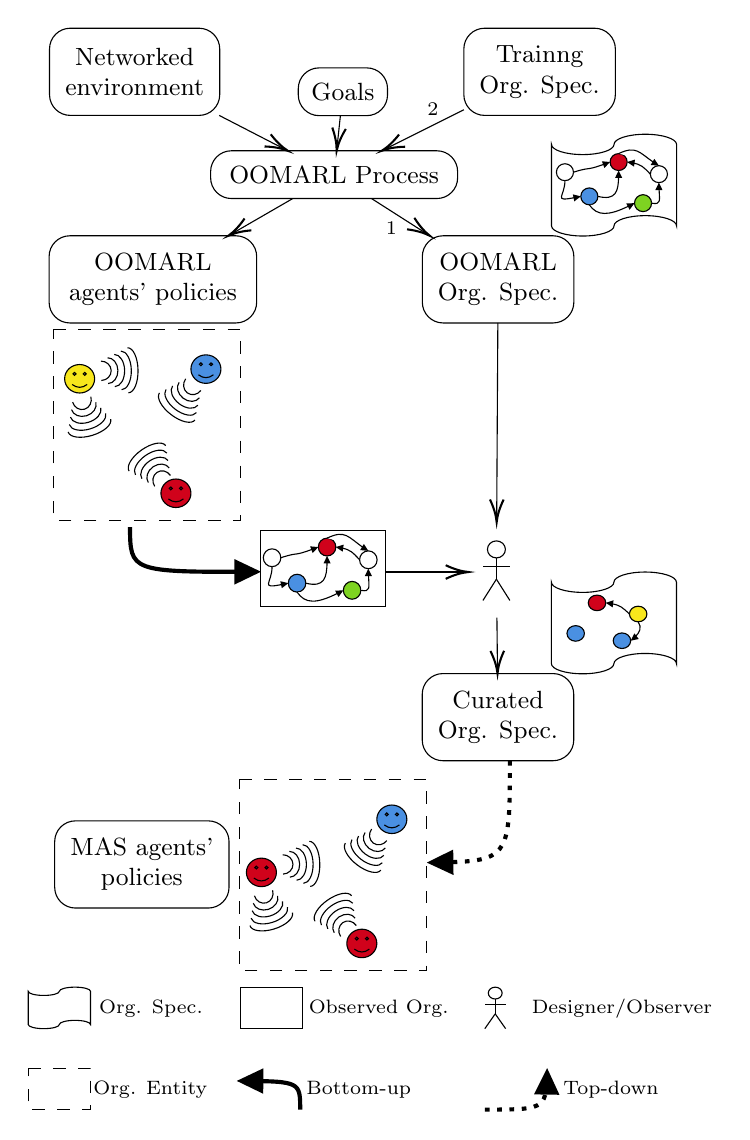
\begin{tikzpicture}[x=0.75pt,y=0.75pt,yscale=-1,xscale=1]
%uncomment if require: \path (0,567); %set diagram left start at 0, and has height of 567

%Flowchart: Punched Tape [id:dp09352793636343182] 
\draw  [fill={rgb, 255:red, 255; green, 255; blue, 255 }  ,fill opacity=1 ] (260,284.9) .. controls (260,287.61) and (266.74,289.81) .. (275.06,289.81) .. controls (283.38,289.81) and (290.12,287.61) .. (290.12,284.9) .. controls (290.12,282.2) and (296.87,280) .. (305.18,280) .. controls (313.5,280) and (320.25,282.2) .. (320.25,284.9) -- (320.25,324.13) .. controls (320.25,321.42) and (313.5,319.23) .. (305.18,319.23) .. controls (296.87,319.23) and (290.12,321.42) .. (290.12,324.13) .. controls (290.12,326.84) and (283.38,329.03) .. (275.06,329.03) .. controls (266.74,329.03) and (260,326.84) .. (260,324.13) -- cycle ;
%Shape: Ellipse [id:dp8537944349912123] 
\draw  [fill={rgb, 255:red, 208; green, 2; blue, 27 }  ,fill opacity=1 ] (277.77,294.86) .. controls (277.77,292.79) and (279.66,291.11) .. (281.98,291.11) .. controls (284.3,291.11) and (286.19,292.79) .. (286.19,294.86) .. controls (286.19,296.94) and (284.3,298.62) .. (281.98,298.62) .. controls (279.66,298.62) and (277.77,296.94) .. (277.77,294.86) -- cycle ;
%Shape: Ellipse [id:dp6897748103188357] 
\draw  [fill={rgb, 255:red, 248; green, 231; blue, 28 }  ,fill opacity=1 ] (297.6,300.23) .. controls (297.6,298.15) and (299.49,296.47) .. (301.81,296.47) .. controls (304.13,296.47) and (306.02,298.15) .. (306.02,300.23) .. controls (306.02,302.3) and (304.13,303.98) .. (301.81,303.98) .. controls (299.49,303.98) and (297.6,302.3) .. (297.6,300.23) -- cycle ;
%Shape: Ellipse [id:dp4802320082509959] 
\draw  [fill={rgb, 255:red, 74; green, 144; blue, 226 }  ,fill opacity=1 ] (289.79,313.09) .. controls (289.79,311.02) and (291.67,309.34) .. (294,309.34) .. controls (296.32,309.34) and (298.2,311.02) .. (298.2,313.09) .. controls (298.2,315.17) and (296.32,316.85) .. (294,316.85) .. controls (291.67,316.85) and (289.79,315.17) .. (289.79,313.09) -- cycle ;
%Curve Lines [id:da7546101861138359] 
\draw [fill={rgb, 255:red, 255; green, 255; blue, 255 }  ,fill opacity=1 ]   (297.6,300.23) .. controls (294.11,296.93) and (293.1,296) .. (289.08,295.29) ;
\draw [shift={(286.19,294.86)}, rotate = 7.39] [fill={rgb, 255:red, 0; green, 0; blue, 0 }  ][line width=0.08]  [draw opacity=0] (3.57,-1.72) -- (0,0) -- (3.57,1.72) -- cycle    ;
%Shape: Ellipse [id:dp693668966316707] 
\draw  [fill={rgb, 255:red, 74; green, 144; blue, 226 }  ,fill opacity=1 ] (267.5,309.58) .. controls (267.5,307.51) and (269.38,305.83) .. (271.71,305.83) .. controls (274.03,305.83) and (275.91,307.51) .. (275.91,309.58) .. controls (275.91,311.65) and (274.03,313.33) .. (271.71,313.33) .. controls (269.38,313.33) and (267.5,311.65) .. (267.5,309.58) -- cycle ;
%Curve Lines [id:da5612242217579502] 
\draw [fill={rgb, 255:red, 255; green, 255; blue, 255 }  ,fill opacity=1 ]   (301.81,303.98) .. controls (303.69,306.69) and (302.57,309.05) .. (300.45,311.16) ;
\draw [shift={(298.2,313.09)}, rotate = 322.38] [fill={rgb, 255:red, 0; green, 0; blue, 0 }  ][line width=0.08]  [draw opacity=0] (3.57,-1.72) -- (0,0) -- (3.57,1.72) -- cycle    ;

%Shape: Rectangle [id:dp7949048767988509] 
\draw  [dash pattern={on 4.5pt off 4.5pt}] (20.05,163.11) -- (110.42,163.11) -- (110.42,255.04) -- (20.05,255.04) -- cycle ;
%Shape: Smiley Face [id:dp8425156316307105] 
\draw  [fill={rgb, 255:red, 248; green, 231; blue, 28 }  ,fill opacity=1 ] (25.48,186.89) .. controls (25.48,183.1) and (28.71,180.03) .. (32.71,180.03) .. controls (36.7,180.03) and (39.94,183.1) .. (39.94,186.89) .. controls (39.94,190.68) and (36.7,193.75) .. (32.71,193.75) .. controls (28.71,193.75) and (25.48,190.68) .. (25.48,186.89) -- cycle ; \draw  [fill={rgb, 255:red, 248; green, 231; blue, 28 }  ,fill opacity=1 ] (29.53,184.56) .. controls (29.53,184.18) and (29.85,183.87) .. (30.25,183.87) .. controls (30.65,183.87) and (30.97,184.18) .. (30.97,184.56) .. controls (30.97,184.94) and (30.65,185.24) .. (30.25,185.24) .. controls (29.85,185.24) and (29.53,184.94) .. (29.53,184.56) -- cycle ; \draw  [fill={rgb, 255:red, 248; green, 231; blue, 28 }  ,fill opacity=1 ] (34.44,184.56) .. controls (34.44,184.18) and (34.77,183.87) .. (35.16,183.87) .. controls (35.56,183.87) and (35.89,184.18) .. (35.89,184.56) .. controls (35.89,184.94) and (35.56,185.24) .. (35.16,185.24) .. controls (34.77,185.24) and (34.44,184.94) .. (34.44,184.56) -- cycle ; \draw   (29.09,189.64) .. controls (31.5,191.47) and (33.91,191.47) .. (36.32,189.64) ;
%Shape: Arc [id:dp7103754459108031] 
\draw  [draw opacity=0] (47.66,206.32) .. controls (47.66,206.32) and (47.66,206.32) .. (47.66,206.32) .. controls (48.43,208.93) and (44.47,212.43) .. (38.81,214.15) .. controls (33.16,215.87) and (27.96,215.15) .. (27.19,212.54) -- (37.43,209.43) -- cycle ; \draw   (47.66,206.32) .. controls (47.66,206.32) and (47.66,206.32) .. (47.66,206.32) .. controls (48.43,208.93) and (44.47,212.43) .. (38.81,214.15) .. controls (33.16,215.87) and (27.96,215.15) .. (27.19,212.54) ;  
%Shape: Arc [id:dp9993647702991559] 
\draw  [draw opacity=0] (45.27,203.61) .. controls (46.04,206.22) and (42.73,209.53) .. (37.89,211) .. controls (33.04,212.48) and (28.49,211.55) .. (27.73,208.94) -- (36.5,206.28) -- cycle ; \draw   (45.27,203.61) .. controls (46.04,206.22) and (42.73,209.53) .. (37.89,211) .. controls (33.04,212.48) and (28.49,211.55) .. (27.73,208.94) ;  
%Shape: Arc [id:dp33021260729129986] 
\draw  [draw opacity=0] (42.88,200.9) .. controls (42.88,200.9) and (42.88,200.9) .. (42.88,200.9) .. controls (43.65,203.51) and (41,206.62) .. (36.96,207.85) .. controls (32.92,209.08) and (29.03,207.96) .. (28.26,205.35) -- (35.57,203.12) -- cycle ; \draw   (42.88,200.9) .. controls (42.88,200.9) and (42.88,200.9) .. (42.88,200.9) .. controls (43.65,203.51) and (41,206.62) .. (36.96,207.85) .. controls (32.92,209.08) and (29.03,207.96) .. (28.26,205.35) ;  
%Shape: Arc [id:dp7515950702187679] 
\draw  [draw opacity=0] (40.5,198.2) .. controls (40.5,198.2) and (40.5,198.2) .. (40.5,198.2) .. controls (40.5,198.2) and (40.5,198.2) .. (40.5,198.2) .. controls (41.26,200.81) and (39.27,203.72) .. (36.04,204.7) .. controls (32.81,205.68) and (29.57,204.36) .. (28.8,201.75) .. controls (28.8,201.75) and (28.8,201.75) .. (28.8,201.75) -- (34.65,199.97) -- cycle ; \draw   (40.5,198.2) .. controls (40.5,198.2) and (40.5,198.2) .. (40.5,198.2) .. controls (40.5,198.2) and (40.5,198.2) .. (40.5,198.2) .. controls (41.26,200.81) and (39.27,203.72) .. (36.04,204.7) .. controls (32.81,205.68) and (29.57,204.36) .. (28.8,201.75) .. controls (28.8,201.75) and (28.8,201.75) .. (28.8,201.75) ;  
%Shape: Arc [id:dp17995425823285305] 
\draw  [draw opacity=0] (38.11,195.49) .. controls (38.11,195.49) and (38.11,195.49) .. (38.11,195.49) .. controls (38.11,195.49) and (38.11,195.49) .. (38.11,195.49) .. controls (38.88,198.1) and (37.53,200.81) .. (35.11,201.55) .. controls (32.69,202.29) and (30.1,200.77) .. (29.34,198.16) -- (33.72,196.82) -- cycle ; \draw   (38.11,195.49) .. controls (38.11,195.49) and (38.11,195.49) .. (38.11,195.49) .. controls (38.11,195.49) and (38.11,195.49) .. (38.11,195.49) .. controls (38.88,198.1) and (37.53,200.81) .. (35.11,201.55) .. controls (32.69,202.29) and (30.1,200.77) .. (29.34,198.16) ;  

%Shape: Arc [id:dp8934563741256025] 
\draw  [draw opacity=0] (55.78,171.93) .. controls (58.46,171.87) and (60.73,176.69) .. (60.84,182.69) .. controls (60.96,188.7) and (58.88,193.6) .. (56.21,193.66) -- (55.99,182.79) -- cycle ; \draw   (55.78,171.93) .. controls (58.46,171.87) and (60.73,176.69) .. (60.84,182.69) .. controls (60.96,188.7) and (58.88,193.6) .. (56.21,193.66) ;  
%Shape: Arc [id:dp5963815446588989] 
\draw  [draw opacity=0] (52.58,173.54) .. controls (55.26,173.49) and (57.51,177.62) .. (57.61,182.76) .. controls (57.71,187.9) and (55.62,192.12) .. (52.94,192.17) -- (52.76,182.86) -- cycle ; \draw   (52.58,173.54) .. controls (55.26,173.49) and (57.51,177.62) .. (57.61,182.76) .. controls (57.71,187.9) and (55.62,192.12) .. (52.94,192.17) ;  
%Shape: Arc [id:dp3378668028957823] 
\draw  [draw opacity=0] (49.38,175.16) .. controls (49.38,175.16) and (49.38,175.16) .. (49.38,175.16) .. controls (49.38,175.16) and (49.38,175.16) .. (49.38,175.16) .. controls (52.06,175.11) and (54.3,178.54) .. (54.38,182.82) .. controls (54.46,187.11) and (52.36,190.63) .. (49.68,190.68) -- (49.53,182.92) -- cycle ; \draw   (49.38,175.16) .. controls (49.38,175.16) and (49.38,175.16) .. (49.38,175.16) .. controls (49.38,175.16) and (49.38,175.16) .. (49.38,175.16) .. controls (52.06,175.11) and (54.3,178.54) .. (54.38,182.82) .. controls (54.46,187.11) and (52.36,190.63) .. (49.68,190.68) ;  
%Shape: Arc [id:dp7870035207223711] 
\draw  [draw opacity=0] (46.18,176.78) .. controls (48.86,176.72) and (51.08,179.46) .. (51.15,182.89) .. controls (51.21,186.32) and (49.1,189.14) .. (46.42,189.2) -- (46.3,182.99) -- cycle ; \draw   (46.18,176.78) .. controls (48.86,176.72) and (51.08,179.46) .. (51.15,182.89) .. controls (51.21,186.32) and (49.1,189.14) .. (46.42,189.2) ;  
%Shape: Arc [id:dp7731275981870975] 
\draw  [draw opacity=0] (42.98,178.39) .. controls (42.98,178.39) and (42.98,178.39) .. (42.98,178.39) .. controls (45.65,178.34) and (47.86,180.38) .. (47.91,182.95) .. controls (47.96,185.53) and (45.83,187.65) .. (43.16,187.71) -- (43.07,183.05) -- cycle ; \draw   (42.98,178.39) .. controls (42.98,178.39) and (42.98,178.39) .. (42.98,178.39) .. controls (45.65,178.34) and (47.86,180.38) .. (47.91,182.95) .. controls (47.96,185.53) and (45.83,187.65) .. (43.16,187.71) ;  

%Shape: Smiley Face [id:dp9460068866596214] 
\draw  [fill={rgb, 255:red, 208; green, 2; blue, 27 }  ,fill opacity=1 ] (71.87,242.05) .. controls (71.87,238.26) and (75.1,235.19) .. (79.1,235.19) .. controls (83.09,235.19) and (86.33,238.26) .. (86.33,242.05) .. controls (86.33,245.84) and (83.09,248.92) .. (79.1,248.92) .. controls (75.1,248.92) and (71.87,245.84) .. (71.87,242.05) -- cycle ; \draw  [fill={rgb, 255:red, 208; green, 2; blue, 27 }  ,fill opacity=1 ] (75.91,239.72) .. controls (75.91,239.34) and (76.24,239.03) .. (76.64,239.03) .. controls (77.04,239.03) and (77.36,239.34) .. (77.36,239.72) .. controls (77.36,240.1) and (77.04,240.4) .. (76.64,240.4) .. controls (76.24,240.4) and (75.91,240.1) .. (75.91,239.72) -- cycle ; \draw  [fill={rgb, 255:red, 208; green, 2; blue, 27 }  ,fill opacity=1 ] (80.83,239.72) .. controls (80.83,239.34) and (81.15,239.03) .. (81.55,239.03) .. controls (81.95,239.03) and (82.28,239.34) .. (82.28,239.72) .. controls (82.28,240.1) and (81.95,240.4) .. (81.55,240.4) .. controls (81.15,240.4) and (80.83,240.1) .. (80.83,239.72) -- cycle ; \draw   (75.48,244.8) .. controls (77.89,246.63) and (80.3,246.63) .. (82.71,244.8) ;
%Shape: Arc [id:dp2662505393390908] 
\draw  [draw opacity=0] (56.53,231.38) .. controls (56.53,231.38) and (56.53,231.38) .. (56.53,231.38) .. controls (56.53,231.38) and (56.53,231.38) .. (56.53,231.38) .. controls (55.02,229.13) and (57.74,224.56) .. (62.6,221.17) .. controls (67.47,217.77) and (72.64,216.84) .. (74.15,219.09) -- (65.34,225.24) -- cycle ; \draw   (56.53,231.38) .. controls (56.53,231.38) and (56.53,231.38) .. (56.53,231.38) .. controls (56.53,231.38) and (56.53,231.38) .. (56.53,231.38) .. controls (55.02,229.13) and (57.74,224.56) .. (62.6,221.17) .. controls (67.47,217.77) and (72.64,216.84) .. (74.15,219.09) ;  
%Shape: Arc [id:dp5533657200850002] 
\draw  [draw opacity=0] (59.62,233.22) .. controls (59.62,233.22) and (59.62,233.22) .. (59.62,233.22) .. controls (58.11,230.97) and (60.26,226.79) .. (64.43,223.88) .. controls (68.6,220.97) and (73.21,220.43) .. (74.72,222.68) -- (67.17,227.95) -- cycle ; \draw   (59.62,233.22) .. controls (59.62,233.22) and (59.62,233.22) .. (59.62,233.22) .. controls (58.11,230.97) and (60.26,226.79) .. (64.43,223.88) .. controls (68.6,220.97) and (73.21,220.43) .. (74.72,222.68) ;  
%Shape: Arc [id:dp130720604660594] 
\draw  [draw opacity=0] (62.71,235.05) .. controls (61.19,232.8) and (62.78,229.02) .. (66.26,226.59) .. controls (69.73,224.17) and (73.78,224.02) .. (75.29,226.27) -- (69,230.66) -- cycle ; \draw   (62.71,235.05) .. controls (61.19,232.8) and (62.78,229.02) .. (66.26,226.59) .. controls (69.73,224.17) and (73.78,224.02) .. (75.29,226.27) ;  
%Shape: Arc [id:dp7777326608896638] 
\draw  [draw opacity=0] (65.79,236.88) .. controls (65.79,236.88) and (65.79,236.88) .. (65.79,236.88) .. controls (64.28,234.64) and (65.31,231.24) .. (68.09,229.3) .. controls (70.87,227.36) and (74.35,227.61) .. (75.86,229.86) -- (70.83,233.37) -- cycle ; \draw   (65.79,236.88) .. controls (65.79,236.88) and (65.79,236.88) .. (65.79,236.88) .. controls (64.28,234.64) and (65.31,231.24) .. (68.09,229.3) .. controls (70.87,227.36) and (74.35,227.61) .. (75.86,229.86) ;  
%Shape: Arc [id:dp4348101062357661] 
\draw  [draw opacity=0] (68.88,238.72) .. controls (67.37,236.47) and (67.83,233.47) .. (69.92,232.02) .. controls (72,230.56) and (74.92,231.2) .. (76.43,233.45) -- (72.66,236.08) -- cycle ; \draw   (68.88,238.72) .. controls (67.37,236.47) and (67.83,233.47) .. (69.92,232.02) .. controls (72,230.56) and (74.92,231.2) .. (76.43,233.45) ;  

%Shape: Smiley Face [id:dp40321958667865143] 
\draw  [fill={rgb, 255:red, 74; green, 144; blue, 226 }  ,fill opacity=1 ] (86.33,182.23) .. controls (86.33,178.44) and (89.56,175.37) .. (93.55,175.37) .. controls (97.55,175.37) and (100.78,178.44) .. (100.78,182.23) .. controls (100.78,186.02) and (97.55,189.1) .. (93.55,189.1) .. controls (89.56,189.1) and (86.33,186.02) .. (86.33,182.23) -- cycle ; \draw  [fill={rgb, 255:red, 74; green, 144; blue, 226 }  ,fill opacity=1 ] (90.37,179.9) .. controls (90.37,179.52) and (90.7,179.21) .. (91.1,179.21) .. controls (91.5,179.21) and (91.82,179.52) .. (91.82,179.9) .. controls (91.82,180.28) and (91.5,180.58) .. (91.1,180.58) .. controls (90.7,180.58) and (90.37,180.28) .. (90.37,179.9) -- cycle ; \draw  [fill={rgb, 255:red, 74; green, 144; blue, 226 }  ,fill opacity=1 ] (95.29,179.9) .. controls (95.29,179.52) and (95.61,179.21) .. (96.01,179.21) .. controls (96.41,179.21) and (96.74,179.52) .. (96.74,179.9) .. controls (96.74,180.28) and (96.41,180.58) .. (96.01,180.58) .. controls (95.61,180.58) and (95.29,180.28) .. (95.29,179.9) -- cycle ; \draw   (89.94,184.98) .. controls (92.35,186.81) and (94.76,186.81) .. (97.17,184.98) ;
%Shape: Arc [id:dp6344973920370733] 
\draw  [draw opacity=0] (88.26,206.75) .. controls (88.26,206.75) and (88.26,206.75) .. (88.26,206.75) .. controls (86.65,208.93) and (81.52,207.78) .. (76.8,204.18) .. controls (72.08,200.58) and (69.55,195.9) .. (71.16,193.72) -- (79.71,200.23) -- cycle ; \draw   (88.26,206.75) .. controls (88.26,206.75) and (88.26,206.75) .. (88.26,206.75) .. controls (86.65,208.93) and (81.52,207.78) .. (76.8,204.18) .. controls (72.08,200.58) and (69.55,195.9) .. (71.16,193.72) ;  
%Shape: Arc [id:dp2502725185770005] 
\draw  [draw opacity=0] (88.97,203.19) .. controls (88.97,203.19) and (88.97,203.19) .. (88.97,203.19) .. controls (88.97,203.19) and (88.97,203.19) .. (88.97,203.19) .. controls (87.37,205.37) and (82.78,204.63) .. (78.74,201.55) .. controls (74.69,198.46) and (72.71,194.2) .. (74.32,192.02) -- (81.65,197.6) -- cycle ; \draw   (88.97,203.19) .. controls (88.97,203.19) and (88.97,203.19) .. (88.97,203.19) .. controls (88.97,203.19) and (88.97,203.19) .. (88.97,203.19) .. controls (87.37,205.37) and (82.78,204.63) .. (78.74,201.55) .. controls (74.69,198.46) and (72.71,194.2) .. (74.32,192.02) ;  
%Shape: Arc [id:dp23421846029392612] 
\draw  [draw opacity=0] (89.69,199.63) .. controls (89.69,199.63) and (89.69,199.63) .. (89.69,199.63) .. controls (89.69,199.63) and (89.69,199.63) .. (89.69,199.63) .. controls (88.08,201.81) and (84.05,201.49) .. (80.68,198.92) .. controls (77.3,196.35) and (75.87,192.5) .. (77.48,190.32) -- (83.58,194.97) -- cycle ; \draw   (89.69,199.63) .. controls (89.69,199.63) and (89.69,199.63) .. (89.69,199.63) .. controls (89.69,199.63) and (89.69,199.63) .. (89.69,199.63) .. controls (88.08,201.81) and (84.05,201.49) .. (80.68,198.92) .. controls (77.3,196.35) and (75.87,192.5) .. (77.48,190.32) ;  
%Shape: Arc [id:dp02946644855410807] 
\draw  [draw opacity=0] (90.41,196.06) .. controls (88.8,198.24) and (85.31,198.34) .. (82.62,196.29) .. controls (79.92,194.23) and (79.03,190.8) .. (80.64,188.62) -- (85.52,192.34) -- cycle ; \draw   (90.41,196.06) .. controls (88.8,198.24) and (85.31,198.34) .. (82.62,196.29) .. controls (79.92,194.23) and (79.03,190.8) .. (80.64,188.62) ;  
%Shape: Arc [id:dp07919277634076938] 
\draw  [draw opacity=0] (91.13,192.5) .. controls (91.13,192.5) and (91.13,192.5) .. (91.13,192.5) .. controls (89.52,194.68) and (86.58,195.2) .. (84.55,193.66) .. controls (82.53,192.11) and (82.19,189.1) .. (83.8,186.92) -- (87.46,189.71) -- cycle ; \draw   (91.13,192.5) .. controls (91.13,192.5) and (91.13,192.5) .. (91.13,192.5) .. controls (89.52,194.68) and (86.58,195.2) .. (84.55,193.66) .. controls (82.53,192.11) and (82.19,189.1) .. (83.8,186.92) ;  

%Shape: Ellipse [id:dp5665300419613197] 
\draw   (229.18,269.1) .. controls (229.18,266.84) and (231.12,265) .. (233.51,265) .. controls (235.9,265) and (237.84,266.84) .. (237.84,269.1) .. controls (237.84,271.36) and (235.9,273.2) .. (233.51,273.2) .. controls (231.12,273.2) and (229.18,271.36) .. (229.18,269.1) -- cycle ;
%Straight Lines [id:da868287133321088] 
\draw    (233.51,273.2) -- (233.51,283.45) ;
%Straight Lines [id:da7338999456859931] 
\draw    (233.51,283.45) -- (227.02,293.7) ;
%Straight Lines [id:da7618645013452761] 
\draw    (233.51,283.45) -- (240,293.7) ;
%Straight Lines [id:da7029210082761028] 
\draw    (240,277.3) -- (227.02,277.3) ;

%Shape: Rectangle [id:dp36259598060414655] 
\draw  [fill={rgb, 255:red, 255; green, 255; blue, 255 }  ,fill opacity=1 ] (120,260) -- (180.25,260) -- (180.25,296.77) -- (120,296.77) -- cycle ;
%Shape: Ellipse [id:dp34598635042601256] 
\draw  [fill={rgb, 255:red, 255; green, 255; blue, 255 }  ,fill opacity=1 ] (121.2,273.12) .. controls (121.2,270.75) and (123.09,268.83) .. (125.42,268.83) .. controls (127.75,268.83) and (129.64,270.75) .. (129.64,273.12) .. controls (129.64,275.49) and (127.75,277.41) .. (125.42,277.41) .. controls (123.09,277.41) and (121.2,275.49) .. (121.2,273.12) -- cycle ;
%Shape: Ellipse [id:dp0011247415244253212] 
\draw  [fill={rgb, 255:red, 74; green, 144; blue, 226 }  ,fill opacity=1 ] (133.25,285.37) .. controls (133.25,283) and (135.14,281.08) .. (137.47,281.08) .. controls (139.8,281.08) and (141.69,283) .. (141.69,285.37) .. controls (141.69,287.74) and (139.8,289.66) .. (137.47,289.66) .. controls (135.14,289.66) and (133.25,287.74) .. (133.25,285.37) -- cycle ;
%Shape: Ellipse [id:dp8822927144483022] 
\draw  [fill={rgb, 255:red, 208; green, 2; blue, 27 }  ,fill opacity=1 ] (147.71,267.97) .. controls (147.71,265.6) and (149.6,263.68) .. (151.93,263.68) .. controls (154.26,263.68) and (156.15,265.6) .. (156.15,267.97) .. controls (156.15,270.34) and (154.26,272.26) .. (151.93,272.26) .. controls (149.6,272.26) and (147.71,270.34) .. (147.71,267.97) -- cycle ;
%Shape: Ellipse [id:dp7611446545020739] 
\draw  [fill={rgb, 255:red, 255; green, 255; blue, 255 }  ,fill opacity=1 ] (167.59,274.1) .. controls (167.59,271.73) and (169.48,269.81) .. (171.81,269.81) .. controls (174.14,269.81) and (176.03,271.73) .. (176.03,274.1) .. controls (176.03,276.47) and (174.14,278.39) .. (171.81,278.39) .. controls (169.48,278.39) and (167.59,276.47) .. (167.59,274.1) -- cycle ;
%Shape: Ellipse [id:dp1592826898001829] 
\draw  [fill={rgb, 255:red, 126; green, 211; blue, 33 }  ,fill opacity=1 ] (159.76,288.81) .. controls (159.76,286.44) and (161.65,284.52) .. (163.98,284.52) .. controls (166.31,284.52) and (168.2,286.44) .. (168.2,288.81) .. controls (168.2,291.18) and (166.31,293.1) .. (163.98,293.1) .. controls (161.65,293.1) and (159.76,291.18) .. (159.76,288.81) -- cycle ;
%Curve Lines [id:da27399536046205264] 
\draw [fill={rgb, 255:red, 255; green, 255; blue, 255 }  ,fill opacity=1 ]   (129.64,273.12) .. controls (139.11,270.05) and (134.67,272.76) .. (144.92,269.01) ;
\draw [shift={(147.71,267.97)}, rotate = 159.17] [fill={rgb, 255:red, 0; green, 0; blue, 0 }  ][line width=0.08]  [draw opacity=0] (3.57,-1.72) -- (0,0) -- (3.57,1.72) -- cycle    ;
%Curve Lines [id:da16623917428090795] 
\draw [fill={rgb, 255:red, 255; green, 255; blue, 255 }  ,fill opacity=1 ]   (141.69,285.37) .. controls (150.75,287.65) and (151.79,282.63) .. (151.91,275.25) ;
\draw [shift={(151.93,272.26)}, rotate = 90] [fill={rgb, 255:red, 0; green, 0; blue, 0 }  ][line width=0.08]  [draw opacity=0] (3.57,-1.72) -- (0,0) -- (3.57,1.72) -- cycle    ;
%Curve Lines [id:da46234775845087284] 
\draw [fill={rgb, 255:red, 255; green, 255; blue, 255 }  ,fill opacity=1 ]   (167.59,274.1) .. controls (164.09,270.33) and (163.08,269.27) .. (159.05,268.46) ;
\draw [shift={(156.15,267.97)}, rotate = 8.42] [fill={rgb, 255:red, 0; green, 0; blue, 0 }  ][line width=0.08]  [draw opacity=0] (3.57,-1.72) -- (0,0) -- (3.57,1.72) -- cycle    ;
%Curve Lines [id:da3119386523209393] 
\draw [fill={rgb, 255:red, 255; green, 255; blue, 255 }  ,fill opacity=1 ]   (168.2,288.81) .. controls (172.97,289.67) and (172.14,287.87) .. (171.87,281.33) ;
\draw [shift={(171.81,278.39)}, rotate = 90] [fill={rgb, 255:red, 0; green, 0; blue, 0 }  ][line width=0.08]  [draw opacity=0] (3.57,-1.72) -- (0,0) -- (3.57,1.72) -- cycle    ;
%Curve Lines [id:da8983756138417751] 
\draw [fill={rgb, 255:red, 255; green, 255; blue, 255 }  ,fill opacity=1 ]   (125.42,277.41) .. controls (125.42,285.5) and (119.17,288.19) .. (130.41,285.96) ;
\draw [shift={(133.25,285.37)}, rotate = 168.05] [fill={rgb, 255:red, 0; green, 0; blue, 0 }  ][line width=0.08]  [draw opacity=0] (3.57,-1.72) -- (0,0) -- (3.57,1.72) -- cycle    ;
%Curve Lines [id:da8579733900345894] 
\draw [fill={rgb, 255:red, 255; green, 255; blue, 255 }  ,fill opacity=1 ]   (137.47,289.66) .. controls (141.37,295.45) and (146.82,295.36) .. (157.15,290.17) ;
\draw [shift={(159.76,288.81)}, rotate = 151.67] [fill={rgb, 255:red, 0; green, 0; blue, 0 }  ][line width=0.08]  [draw opacity=0] (3.57,-1.72) -- (0,0) -- (3.57,1.72) -- cycle    ;
%Curve Lines [id:da598997074659714] 
\draw [fill={rgb, 255:red, 255; green, 255; blue, 255 }  ,fill opacity=1 ]   (151.93,263.68) .. controls (160.7,259.44) and (161.99,263.12) .. (169.42,268.25) ;
\draw [shift={(171.81,269.81)}, rotate = 211.4] [fill={rgb, 255:red, 0; green, 0; blue, 0 }  ][line width=0.08]  [draw opacity=0] (3.57,-1.72) -- (0,0) -- (3.57,1.72) -- cycle    ;

%Shape: Boxed Bezier Curve [id:dp04329100663395624] 
\draw [line width=1.5]    (56.97,258.4) .. controls (57.12,279.64) and (57.12,280.06) .. (116.36,279.88) ;
\draw [shift={(120.07,279.86)}, rotate = 179.81] [fill={rgb, 255:red, 0; green, 0; blue, 0 }  ][line width=0.08]  [draw opacity=0] (12.77,-6.13) -- (0,0) -- (12.77,6.13) -- cycle    ;
%Shape: Boxed Bezier Curve [id:dp3249540323733473] 
\draw [line width=1.5]  [dash pattern={on 1.69pt off 2.76pt}]  (240,371) .. controls (240,377.31) and (240,382.8) .. (239.91,387.58) .. controls (239.34,418.4) and (235.11,419.53) .. (203.54,419.96) ;
\draw [shift={(200,420)}, rotate = 359.3] [fill={rgb, 255:red, 0; green, 0; blue, 0 }  ][line width=0.08]  [draw opacity=0] (12.77,-6.13) -- (0,0) -- (12.77,6.13) -- cycle    ;
%Shape: Rectangle [id:dp3591393250200341] 
\draw  [dash pattern={on 4.5pt off 4.5pt}] (109.63,380) -- (200,380) -- (200,471.94) -- (109.63,471.94) -- cycle ;
%Shape: Smiley Face [id:dp3801591887945033] 
\draw  [fill={rgb, 255:red, 208; green, 2; blue, 27 }  ,fill opacity=1 ] (113.05,424.72) .. controls (113.05,420.92) and (116.29,417.85) .. (120.28,417.85) .. controls (124.28,417.85) and (127.51,420.92) .. (127.51,424.72) .. controls (127.51,428.51) and (124.28,431.58) .. (120.28,431.58) .. controls (116.29,431.58) and (113.05,428.51) .. (113.05,424.72) -- cycle ; \draw  [fill={rgb, 255:red, 208; green, 2; blue, 27 }  ,fill opacity=1 ] (117.1,422.38) .. controls (117.1,422) and (117.43,421.7) .. (117.82,421.7) .. controls (118.22,421.7) and (118.55,422) .. (118.55,422.38) .. controls (118.55,422.76) and (118.22,423.07) .. (117.82,423.07) .. controls (117.43,423.07) and (117.1,422.76) .. (117.1,422.38) -- cycle ; \draw  [fill={rgb, 255:red, 208; green, 2; blue, 27 }  ,fill opacity=1 ] (122.02,422.38) .. controls (122.02,422) and (122.34,421.7) .. (122.74,421.7) .. controls (123.14,421.7) and (123.46,422) .. (123.46,422.38) .. controls (123.46,422.76) and (123.14,423.07) .. (122.74,423.07) .. controls (122.34,423.07) and (122.02,422.76) .. (122.02,422.38) -- cycle ; \draw   (116.67,427.46) .. controls (119.08,429.29) and (121.49,429.29) .. (123.9,427.46) ;
%Shape: Arc [id:dp40222913228483237] 
\draw  [draw opacity=0] (135.24,444.14) .. controls (135.24,444.14) and (135.24,444.14) .. (135.24,444.14) .. controls (136,446.75) and (132.04,450.26) .. (126.39,451.98) .. controls (120.74,453.7) and (115.53,452.97) .. (114.77,450.36) -- (125,447.25) -- cycle ; \draw   (135.24,444.14) .. controls (135.24,444.14) and (135.24,444.14) .. (135.24,444.14) .. controls (136,446.75) and (132.04,450.26) .. (126.39,451.98) .. controls (120.74,453.7) and (115.53,452.97) .. (114.77,450.36) ;  
%Shape: Arc [id:dp6185790641450695] 
\draw  [draw opacity=0] (132.85,441.43) .. controls (133.62,444.05) and (130.31,447.36) .. (125.46,448.83) .. controls (120.62,450.3) and (116.07,449.38) .. (115.3,446.77) -- (124.08,444.1) -- cycle ; \draw   (132.85,441.43) .. controls (133.62,444.05) and (130.31,447.36) .. (125.46,448.83) .. controls (120.62,450.3) and (116.07,449.38) .. (115.3,446.77) ;  
%Shape: Arc [id:dp6749114191148724] 
\draw  [draw opacity=0] (130.46,438.73) .. controls (130.46,438.73) and (130.46,438.73) .. (130.46,438.73) .. controls (131.23,441.34) and (128.58,444.45) .. (124.54,445.68) .. controls (120.5,446.9) and (116.61,445.78) .. (115.84,443.17) -- (123.15,440.95) -- cycle ; \draw   (130.46,438.73) .. controls (130.46,438.73) and (130.46,438.73) .. (130.46,438.73) .. controls (131.23,441.34) and (128.58,444.45) .. (124.54,445.68) .. controls (120.5,446.9) and (116.61,445.78) .. (115.84,443.17) ;  
%Shape: Arc [id:dp056403546095020296] 
\draw  [draw opacity=0] (128.07,436.02) .. controls (128.07,436.02) and (128.07,436.02) .. (128.07,436.02) .. controls (128.07,436.02) and (128.07,436.02) .. (128.07,436.02) .. controls (128.84,438.63) and (126.84,441.54) .. (123.61,442.53) .. controls (120.38,443.51) and (117.14,442.19) .. (116.38,439.58) -- (122.22,437.8) -- cycle ; \draw   (128.07,436.02) .. controls (128.07,436.02) and (128.07,436.02) .. (128.07,436.02) .. controls (128.07,436.02) and (128.07,436.02) .. (128.07,436.02) .. controls (128.84,438.63) and (126.84,441.54) .. (123.61,442.53) .. controls (120.38,443.51) and (117.14,442.19) .. (116.38,439.58) ;  
%Shape: Arc [id:dp048963270262922354] 
\draw  [draw opacity=0] (125.69,433.32) .. controls (125.69,433.32) and (125.69,433.32) .. (125.69,433.32) .. controls (126.45,435.93) and (125.11,438.64) .. (122.69,439.38) .. controls (120.27,440.11) and (117.68,438.59) .. (116.91,435.98) -- (121.3,434.65) -- cycle ; \draw   (125.69,433.32) .. controls (125.69,433.32) and (125.69,433.32) .. (125.69,433.32) .. controls (126.45,435.93) and (125.11,438.64) .. (122.69,439.38) .. controls (120.27,440.11) and (117.68,438.59) .. (116.91,435.98) ;  

%Shape: Arc [id:dp11791815378481285] 
\draw  [draw opacity=0] (143.36,409.75) .. controls (143.36,409.75) and (143.36,409.75) .. (143.36,409.75) .. controls (146.04,409.7) and (148.3,414.52) .. (148.42,420.52) .. controls (148.54,426.52) and (146.46,431.43) .. (143.78,431.48) -- (143.57,420.62) -- cycle ; \draw   (143.36,409.75) .. controls (143.36,409.75) and (143.36,409.75) .. (143.36,409.75) .. controls (146.04,409.7) and (148.3,414.52) .. (148.42,420.52) .. controls (148.54,426.52) and (146.46,431.43) .. (143.78,431.48) ;  
%Shape: Arc [id:dp6186444432706435] 
\draw  [draw opacity=0] (140.16,411.37) .. controls (142.84,411.32) and (145.09,415.44) .. (145.19,420.59) .. controls (145.29,425.73) and (143.2,429.94) .. (140.52,430) -- (140.34,420.68) -- cycle ; \draw   (140.16,411.37) .. controls (142.84,411.32) and (145.09,415.44) .. (145.19,420.59) .. controls (145.29,425.73) and (143.2,429.94) .. (140.52,430) ;  
%Shape: Arc [id:dp3524256769019909] 
\draw  [draw opacity=0] (136.96,412.99) .. controls (136.96,412.99) and (136.96,412.99) .. (136.96,412.99) .. controls (139.63,412.93) and (141.87,416.36) .. (141.96,420.65) .. controls (142.04,424.94) and (139.94,428.45) .. (137.26,428.51) .. controls (137.26,428.51) and (137.26,428.51) .. (137.26,428.51) -- (137.11,420.75) -- cycle ; \draw   (136.96,412.99) .. controls (136.96,412.99) and (136.96,412.99) .. (136.96,412.99) .. controls (139.63,412.93) and (141.87,416.36) .. (141.96,420.65) .. controls (142.04,424.94) and (139.94,428.45) .. (137.26,428.51) .. controls (137.26,428.51) and (137.26,428.51) .. (137.26,428.51) ;  
%Shape: Arc [id:dp9364872182962407] 
\draw  [draw opacity=0] (133.76,414.6) .. controls (136.43,414.55) and (138.66,417.29) .. (138.72,420.72) .. controls (138.79,424.14) and (136.67,426.97) .. (134,427.02) -- (133.88,420.81) -- cycle ; \draw   (133.76,414.6) .. controls (136.43,414.55) and (138.66,417.29) .. (138.72,420.72) .. controls (138.79,424.14) and (136.67,426.97) .. (134,427.02) ;  
%Shape: Arc [id:dp43568764349824574] 
\draw  [draw opacity=0] (130.55,416.22) .. controls (130.55,416.22) and (130.55,416.22) .. (130.55,416.22) .. controls (133.23,416.17) and (135.44,418.21) .. (135.49,420.78) .. controls (135.54,423.35) and (133.41,425.48) .. (130.73,425.53) .. controls (130.73,425.53) and (130.73,425.53) .. (130.73,425.53) -- (130.64,420.88) -- cycle ; \draw   (130.55,416.22) .. controls (130.55,416.22) and (130.55,416.22) .. (130.55,416.22) .. controls (133.23,416.17) and (135.44,418.21) .. (135.49,420.78) .. controls (135.54,423.35) and (133.41,425.48) .. (130.73,425.53) .. controls (130.73,425.53) and (130.73,425.53) .. (130.73,425.53) ;  

%Shape: Smiley Face [id:dp7641236455099758] 
\draw  [fill={rgb, 255:red, 208; green, 2; blue, 27 }  ,fill opacity=1 ] (161.44,458.94) .. controls (161.44,455.15) and (164.68,452.08) .. (168.67,452.08) .. controls (172.66,452.08) and (175.9,455.15) .. (175.9,458.94) .. controls (175.9,462.73) and (172.66,465.81) .. (168.67,465.81) .. controls (164.68,465.81) and (161.44,462.73) .. (161.44,458.94) -- cycle ; \draw  [fill={rgb, 255:red, 208; green, 2; blue, 27 }  ,fill opacity=1 ] (165.49,456.61) .. controls (165.49,456.23) and (165.81,455.92) .. (166.21,455.92) .. controls (166.61,455.92) and (166.94,456.23) .. (166.94,456.61) .. controls (166.94,456.99) and (166.61,457.29) .. (166.21,457.29) .. controls (165.81,457.29) and (165.49,456.99) .. (165.49,456.61) -- cycle ; \draw  [fill={rgb, 255:red, 208; green, 2; blue, 27 }  ,fill opacity=1 ] (170.41,456.61) .. controls (170.41,456.23) and (170.73,455.92) .. (171.13,455.92) .. controls (171.53,455.92) and (171.85,456.23) .. (171.85,456.61) .. controls (171.85,456.99) and (171.53,457.29) .. (171.13,457.29) .. controls (170.73,457.29) and (170.41,456.99) .. (170.41,456.61) -- cycle ; \draw   (165.06,461.69) .. controls (167.47,463.52) and (169.88,463.52) .. (172.29,461.69) ;
%Shape: Arc [id:dp12338485660705834] 
\draw  [draw opacity=0] (146.11,448.27) .. controls (146.11,448.27) and (146.11,448.27) .. (146.11,448.27) .. controls (144.6,446.02) and (147.31,441.45) .. (152.18,438.06) .. controls (157.04,434.66) and (162.22,433.73) .. (163.73,435.98) -- (154.92,442.13) -- cycle ; \draw   (146.11,448.27) .. controls (146.11,448.27) and (146.11,448.27) .. (146.11,448.27) .. controls (144.6,446.02) and (147.31,441.45) .. (152.18,438.06) .. controls (157.04,434.66) and (162.22,433.73) .. (163.73,435.98) ;  
%Shape: Arc [id:dp047340824310728946] 
\draw  [draw opacity=0] (149.2,450.11) .. controls (149.2,450.11) and (149.2,450.11) .. (149.2,450.11) .. controls (147.68,447.86) and (149.84,443.68) .. (154.01,440.77) .. controls (158.18,437.86) and (162.79,437.32) .. (164.3,439.57) -- (156.75,444.84) -- cycle ; \draw   (149.2,450.11) .. controls (149.2,450.11) and (149.2,450.11) .. (149.2,450.11) .. controls (147.68,447.86) and (149.84,443.68) .. (154.01,440.77) .. controls (158.18,437.86) and (162.79,437.32) .. (164.3,439.57) ;  
%Shape: Arc [id:dp5460583680593605] 
\draw  [draw opacity=0] (152.28,451.94) .. controls (150.77,449.69) and (152.36,445.91) .. (155.84,443.48) .. controls (159.31,441.06) and (163.36,440.91) .. (164.87,443.16) -- (158.58,447.55) -- cycle ; \draw   (152.28,451.94) .. controls (150.77,449.69) and (152.36,445.91) .. (155.84,443.48) .. controls (159.31,441.06) and (163.36,440.91) .. (164.87,443.16) ;  
%Shape: Arc [id:dp9281425971103023] 
\draw  [draw opacity=0] (155.37,453.77) .. controls (155.37,453.77) and (155.37,453.77) .. (155.37,453.77) .. controls (153.86,451.53) and (154.88,448.13) .. (157.66,446.19) .. controls (160.44,444.25) and (163.93,444.5) .. (165.44,446.75) -- (160.41,450.26) -- cycle ; \draw   (155.37,453.77) .. controls (155.37,453.77) and (155.37,453.77) .. (155.37,453.77) .. controls (153.86,451.53) and (154.88,448.13) .. (157.66,446.19) .. controls (160.44,444.25) and (163.93,444.5) .. (165.44,446.75) ;  
%Shape: Arc [id:dp6708756452099565] 
\draw  [draw opacity=0] (158.46,455.61) .. controls (158.46,455.61) and (158.46,455.61) .. (158.46,455.61) .. controls (156.94,453.36) and (157.41,450.36) .. (159.49,448.91) .. controls (161.58,447.45) and (164.49,448.09) .. (166.01,450.34) -- (162.23,452.98) -- cycle ; \draw   (158.46,455.61) .. controls (158.46,455.61) and (158.46,455.61) .. (158.46,455.61) .. controls (156.94,453.36) and (157.41,450.36) .. (159.49,448.91) .. controls (161.58,447.45) and (164.49,448.09) .. (166.01,450.34) ;  

%Shape: Smiley Face [id:dp8284136369467816] 
\draw  [fill={rgb, 255:red, 74; green, 144; blue, 226 }  ,fill opacity=1 ] (175.9,399.12) .. controls (175.9,395.33) and (179.14,392.26) .. (183.13,392.26) .. controls (187.12,392.26) and (190.36,395.33) .. (190.36,399.12) .. controls (190.36,402.91) and (187.12,405.99) .. (183.13,405.99) .. controls (179.14,405.99) and (175.9,402.91) .. (175.9,399.12) -- cycle ; \draw  [fill={rgb, 255:red, 74; green, 144; blue, 226 }  ,fill opacity=1 ] (179.95,396.79) .. controls (179.95,396.41) and (180.27,396.1) .. (180.67,396.1) .. controls (181.07,396.1) and (181.4,396.41) .. (181.4,396.79) .. controls (181.4,397.17) and (181.07,397.48) .. (180.67,397.48) .. controls (180.27,397.48) and (179.95,397.17) .. (179.95,396.79) -- cycle ; \draw  [fill={rgb, 255:red, 74; green, 144; blue, 226 }  ,fill opacity=1 ] (184.87,396.79) .. controls (184.87,396.41) and (185.19,396.1) .. (185.59,396.1) .. controls (185.99,396.1) and (186.31,396.41) .. (186.31,396.79) .. controls (186.31,397.17) and (185.99,397.48) .. (185.59,397.48) .. controls (185.19,397.48) and (184.87,397.17) .. (184.87,396.79) -- cycle ; \draw   (179.52,401.87) .. controls (181.93,403.7) and (184.34,403.7) .. (186.75,401.87) ;
%Shape: Arc [id:dp8977395703020796] 
\draw  [draw opacity=0] (177.83,423.64) .. controls (177.83,423.64) and (177.83,423.64) .. (177.83,423.64) .. controls (176.23,425.82) and (171.1,424.67) .. (166.38,421.07) .. controls (161.66,417.47) and (159.13,412.79) .. (160.74,410.61) -- (169.28,417.13) -- cycle ; \draw   (177.83,423.64) .. controls (177.83,423.64) and (177.83,423.64) .. (177.83,423.64) .. controls (176.23,425.82) and (171.1,424.67) .. (166.38,421.07) .. controls (161.66,417.47) and (159.13,412.79) .. (160.74,410.61) ;  
%Shape: Arc [id:dp38070292756653834] 
\draw  [draw opacity=0] (178.55,420.08) .. controls (178.55,420.08) and (178.55,420.08) .. (178.55,420.08) .. controls (178.55,420.08) and (178.55,420.08) .. (178.55,420.08) .. controls (176.94,422.26) and (172.36,421.53) .. (168.31,418.44) .. controls (164.27,415.36) and (162.29,411.09) .. (163.9,408.91) -- (171.22,414.49) -- cycle ; \draw   (178.55,420.08) .. controls (178.55,420.08) and (178.55,420.08) .. (178.55,420.08) .. controls (178.55,420.08) and (178.55,420.08) .. (178.55,420.08) .. controls (176.94,422.26) and (172.36,421.53) .. (168.31,418.44) .. controls (164.27,415.36) and (162.29,411.09) .. (163.9,408.91) ;  
%Shape: Arc [id:dp6719893406275441] 
\draw  [draw opacity=0] (179.27,416.52) .. controls (177.66,418.7) and (173.63,418.38) .. (170.25,415.81) .. controls (166.88,413.24) and (165.45,409.39) .. (167.06,407.21) -- (173.16,411.86) -- cycle ; \draw   (179.27,416.52) .. controls (177.66,418.7) and (173.63,418.38) .. (170.25,415.81) .. controls (166.88,413.24) and (165.45,409.39) .. (167.06,407.21) ;  
%Shape: Arc [id:dp8811123580129818] 
\draw  [draw opacity=0] (179.98,412.95) .. controls (178.38,415.13) and (174.89,415.23) .. (172.19,413.18) .. controls (169.49,411.12) and (168.61,407.69) .. (170.22,405.51) -- (175.1,409.23) -- cycle ; \draw   (179.98,412.95) .. controls (178.38,415.13) and (174.89,415.23) .. (172.19,413.18) .. controls (169.49,411.12) and (168.61,407.69) .. (170.22,405.51) ;  
%Shape: Arc [id:dp008168376750506745] 
\draw  [draw opacity=0] (180.7,409.39) .. controls (179.1,411.57) and (176.15,412.09) .. (174.13,410.55) .. controls (172.11,409) and (171.77,405.99) .. (173.38,403.81) -- (177.04,406.6) -- cycle ; \draw   (180.7,409.39) .. controls (179.1,411.57) and (176.15,412.09) .. (174.13,410.55) .. controls (172.11,409) and (171.77,405.99) .. (173.38,403.81) ;  

%Flowchart: Punched Tape [id:dp3402123777548822] 
\draw  [fill={rgb, 255:red, 255; green, 255; blue, 255 }  ,fill opacity=1 ] (7.94,482) .. controls (7.94,483.1) and (11.3,484) .. (15.44,484) .. controls (19.58,484) and (22.94,483.1) .. (22.94,482) .. controls (22.94,480.9) and (26.3,480) .. (30.44,480) .. controls (34.58,480) and (37.94,480.9) .. (37.94,482) -- (37.94,498) .. controls (37.94,496.9) and (34.58,496) .. (30.44,496) .. controls (26.3,496) and (22.94,496.9) .. (22.94,498) .. controls (22.94,499.1) and (19.58,500) .. (15.44,500) .. controls (11.3,500) and (7.94,499.1) .. (7.94,498) -- cycle ;
%Shape: Rectangle [id:dp5542564540555983] 
\draw  [dash pattern={on 4.5pt off 4.5pt}] (7.94,519) -- (37.94,519) -- (37.94,539) -- (7.94,539) -- cycle ;
%Shape: Ellipse [id:dp5593235195310067] 
\draw   (229.6,482.86) .. controls (229.6,481.28) and (231.1,480) .. (232.94,480) .. controls (234.78,480) and (236.27,481.28) .. (236.27,482.86) .. controls (236.27,484.44) and (234.78,485.71) .. (232.94,485.71) .. controls (231.1,485.71) and (229.6,484.44) .. (229.6,482.86) -- cycle ;
%Straight Lines [id:da12195011989321491] 
\draw    (232.94,485.71) -- (232.94,492.86) ;
%Straight Lines [id:da9713687192344966] 
\draw    (232.94,492.86) -- (227.94,500) ;
%Straight Lines [id:da9227495247808029] 
\draw    (232.94,492.86) -- (237.94,500) ;
%Straight Lines [id:da9436032646867678] 
\draw    (237.94,488.57) -- (227.94,488.57) ;

%Shape: Boxed Bezier Curve [id:dp6746038394007414] 
\draw [line width=1.5]  [dash pattern={on 1.69pt off 2.76pt}]  (227.94,539) .. controls (255.56,539) and (257.49,539) .. (257.87,522.91) ;
\draw [shift={(257.94,519)}, rotate = 90.86] [fill={rgb, 255:red, 0; green, 0; blue, 0 }  ][line width=0.08]  [draw opacity=0] (12.77,-6.13) -- (0,0) -- (12.77,6.13) -- cycle    ;
%Shape: Boxed Bezier Curve [id:dp8252767880244336] 
\draw [line width=1.5]    (138.97,539) .. controls (138.97,525.94) and (138.97,525.35) .. (112.36,525.2) ;
\draw [shift={(108.42,525.18)}, rotate = 0.26] [fill={rgb, 255:red, 0; green, 0; blue, 0 }  ][line width=0.08]  [draw opacity=0] (12.77,-6.13) -- (0,0) -- (12.77,6.13) -- cycle    ;
%Flowchart: Punched Tape [id:dp1596519476860545] 
\draw  [fill={rgb, 255:red, 255; green, 255; blue, 255 }  ,fill opacity=1 ] (260.05,73.98) .. controls (260.05,76.69) and (266.8,78.88) .. (275.12,78.88) .. controls (283.43,78.88) and (290.18,76.69) .. (290.18,73.98) .. controls (290.18,71.27) and (296.92,69.08) .. (305.24,69.08) .. controls (313.56,69.08) and (320.3,71.27) .. (320.3,73.98) -- (320.3,113.21) .. controls (320.3,110.5) and (313.56,108.3) .. (305.24,108.3) .. controls (296.92,108.3) and (290.18,110.5) .. (290.18,113.21) .. controls (290.18,115.91) and (283.43,118.11) .. (275.12,118.11) .. controls (266.8,118.11) and (260.05,115.91) .. (260.05,113.21) -- cycle ;
%Shape: Ellipse [id:dp002685494295735058] 
\draw  [fill={rgb, 255:red, 255; green, 255; blue, 255 }  ,fill opacity=1 ] (262.41,87.37) .. controls (262.41,85.11) and (264.25,83.29) .. (266.52,83.29) .. controls (268.8,83.29) and (270.64,85.11) .. (270.64,87.37) .. controls (270.64,89.62) and (268.8,91.44) .. (266.52,91.44) .. controls (264.25,91.44) and (262.41,89.62) .. (262.41,87.37) -- cycle ;
%Shape: Ellipse [id:dp18321883985201803] 
\draw  [fill={rgb, 255:red, 74; green, 144; blue, 226 }  ,fill opacity=1 ] (274.17,99.02) .. controls (274.17,96.76) and (276.01,94.94) .. (278.28,94.94) .. controls (280.56,94.94) and (282.4,96.76) .. (282.4,99.02) .. controls (282.4,101.27) and (280.56,103.09) .. (278.28,103.09) .. controls (276.01,103.09) and (274.17,101.27) .. (274.17,99.02) -- cycle ;
%Shape: Ellipse [id:dp4076602785297232] 
\draw  [fill={rgb, 255:red, 208; green, 2; blue, 27 }  ,fill opacity=1 ] (288.28,82.47) .. controls (288.28,80.22) and (290.12,78.4) .. (292.4,78.4) .. controls (294.67,78.4) and (296.51,80.22) .. (296.51,82.47) .. controls (296.51,84.73) and (294.67,86.55) .. (292.4,86.55) .. controls (290.12,86.55) and (288.28,84.73) .. (288.28,82.47) -- cycle ;
%Shape: Ellipse [id:dp9213295790384606] 
\draw  [fill={rgb, 255:red, 255; green, 255; blue, 255 }  ,fill opacity=1 ] (307.68,88.3) .. controls (307.68,86.05) and (309.53,84.22) .. (311.8,84.22) .. controls (314.07,84.22) and (315.92,86.05) .. (315.92,88.3) .. controls (315.92,90.55) and (314.07,92.38) .. (311.8,92.38) .. controls (309.53,92.38) and (307.68,90.55) .. (307.68,88.3) -- cycle ;
%Shape: Ellipse [id:dp07303077783269196] 
\draw  [fill={rgb, 255:red, 126; green, 211; blue, 33 }  ,fill opacity=1 ] (300.04,102.28) .. controls (300.04,100.03) and (301.88,98.2) .. (304.16,98.2) .. controls (306.43,98.2) and (308.27,100.03) .. (308.27,102.28) .. controls (308.27,104.53) and (306.43,106.35) .. (304.16,106.35) .. controls (301.88,106.35) and (300.04,104.53) .. (300.04,102.28) -- cycle ;
%Curve Lines [id:da40084119138850793] 
\draw [fill={rgb, 255:red, 255; green, 255; blue, 255 }  ,fill opacity=1 ]   (270.64,87.37) .. controls (279.89,84.46) and (275.55,87.03) .. (285.55,83.47) ;
\draw [shift={(288.28,82.47)}, rotate = 159.68] [fill={rgb, 255:red, 0; green, 0; blue, 0 }  ][line width=0.08]  [draw opacity=0] (3.57,-1.72) -- (0,0) -- (3.57,1.72) -- cycle    ;
%Curve Lines [id:da056316075040988345] 
\draw [fill={rgb, 255:red, 255; green, 255; blue, 255 }  ,fill opacity=1 ]   (282.4,99.02) .. controls (291.2,101.17) and (292.25,96.46) .. (292.38,89.51) ;
\draw [shift={(292.4,86.55)}, rotate = 90] [fill={rgb, 255:red, 0; green, 0; blue, 0 }  ][line width=0.08]  [draw opacity=0] (3.57,-1.72) -- (0,0) -- (3.57,1.72) -- cycle    ;
%Curve Lines [id:da9750985583942122] 
\draw [fill={rgb, 255:red, 255; green, 255; blue, 255 }  ,fill opacity=1 ]   (307.68,88.3) .. controls (304.29,84.74) and (303.29,83.72) .. (299.42,82.95) ;
\draw [shift={(296.51,82.47)}, rotate = 8.2] [fill={rgb, 255:red, 0; green, 0; blue, 0 }  ][line width=0.08]  [draw opacity=0] (3.57,-1.72) -- (0,0) -- (3.57,1.72) -- cycle    ;
%Curve Lines [id:da6143174667543494] 
\draw [fill={rgb, 255:red, 255; green, 255; blue, 255 }  ,fill opacity=1 ]   (308.27,102.28) .. controls (312.9,103.09) and (312.13,101.41) .. (311.87,95.28) ;
\draw [shift={(311.8,92.38)}, rotate = 90] [fill={rgb, 255:red, 0; green, 0; blue, 0 }  ][line width=0.08]  [draw opacity=0] (3.57,-1.72) -- (0,0) -- (3.57,1.72) -- cycle    ;
%Curve Lines [id:da2385044516658259] 
\draw [fill={rgb, 255:red, 255; green, 255; blue, 255 }  ,fill opacity=1 ]   (266.52,91.44) .. controls (266.52,99.14) and (260.42,101.69) .. (271.39,99.57) ;
\draw [shift={(274.17,99.02)}, rotate = 168.36] [fill={rgb, 255:red, 0; green, 0; blue, 0 }  ][line width=0.08]  [draw opacity=0] (3.57,-1.72) -- (0,0) -- (3.57,1.72) -- cycle    ;
%Curve Lines [id:da43759757255400467] 
\draw [fill={rgb, 255:red, 255; green, 255; blue, 255 }  ,fill opacity=1 ]   (278.28,103.09) .. controls (282.09,108.59) and (287.41,108.5) .. (297.49,103.57) ;
\draw [shift={(300.04,102.28)}, rotate = 152.3] [fill={rgb, 255:red, 0; green, 0; blue, 0 }  ][line width=0.08]  [draw opacity=0] (3.57,-1.72) -- (0,0) -- (3.57,1.72) -- cycle    ;
%Curve Lines [id:da6953413668483659] 
\draw [fill={rgb, 255:red, 255; green, 255; blue, 255 }  ,fill opacity=1 ]   (292.4,78.4) .. controls (300.91,74.39) and (302.2,77.83) .. (309.34,82.66) ;
\draw [shift={(311.8,84.22)}, rotate = 210.72] [fill={rgb, 255:red, 0; green, 0; blue, 0 }  ][line width=0.08]  [draw opacity=0] (3.57,-1.72) -- (0,0) -- (3.57,1.72) -- cycle    ;

%Shape: Rectangle [id:dp9331446837705206] 
\draw   (110.07,480) -- (140.07,480) -- (140.07,500) -- (110.07,500) -- cycle ;
%Straight Lines [id:da26229660491858264] 
\draw    (180,280) -- (218,280) ;
\draw [shift={(220,280)}, rotate = 180] [color={rgb, 255:red, 0; green, 0; blue, 0 }  ][line width=0.75]    (10.93,-3.29) .. controls (6.95,-1.4) and (3.31,-0.3) .. (0,0) .. controls (3.31,0.3) and (6.95,1.4) .. (10.93,3.29)   ;


% Text Node
\draw (176.81,490.5) node   [align=left] {{\scriptsize Observed Org.}};
% Text Node
\draw    (197.77,338.92) .. controls (197.77,333.4) and (202.24,328.92) .. (207.77,328.92) -- (260.77,328.92) .. controls (266.29,328.92) and (270.77,333.4) .. (270.77,338.92) -- (270.77,360.92) .. controls (270.77,366.45) and (266.29,370.92) .. (260.77,370.92) -- (207.77,370.92) .. controls (202.24,370.92) and (197.77,366.45) .. (197.77,360.92) -- cycle  ;
\draw (234.27,349.92) node  [font=\small] [align=left] {\begin{minipage}[lt]{46.6pt}\setlength\topsep{0pt}
\begin{center}
Curated\\Org. Spec.
\end{center}

\end{minipage}};
% Text Node
\draw (288.7,529.5) node   [align=left] {{\scriptsize Top-down}};
% Text Node
\draw (167.19,529.5) node   [align=left] {{\scriptsize Bottom-up}};
% Text Node
\draw (294,490.5) node   [align=left] {{\scriptsize Designer/Observer}};
% Text Node
\draw (66.74,529.5) node   [align=left] {{\scriptsize Org. Entity}};
% Text Node
\draw (67.04,490.5) node   [align=left] {{\scriptsize Org. Spec.}};
% Text Node
\draw (199,53) node [anchor=north west][inner sep=0.75pt]   [align=left] {$\displaystyle ^{2}$};
% Text Node
% \draw (179,97) node [anchor=north west][inner sep=0.75pt]   [align=left] {$\displaystyle ^{1}$};
\draw (179,110) node [anchor=north west][inner sep=0.75pt]   [align=left] {$\displaystyle ^{1}$};
% Text Node
\draw    (20.69,409.89) .. controls (20.69,404.37) and (25.17,399.89) .. (30.69,399.89) -- (94.69,399.89) .. controls (100.22,399.89) and (104.69,404.37) .. (104.69,409.89) -- (104.69,431.89) .. controls (104.69,437.41) and (100.22,441.89) .. (94.69,441.89) -- (30.69,441.89) .. controls (25.17,441.89) and (20.69,437.41) .. (20.69,431.89) -- cycle  ;
\draw (62.69,420.89) node  [font=\small] [align=left] {\begin{minipage}[lt]{54.49pt}\setlength\topsep{0pt}
\begin{center}
MAS agents'\\policies
\end{center}

\end{minipage}};
% Text Node
\draw (226,257) node [anchor=north west][inner sep=0.75pt]   [align=left] {\begin{minipage}[lt]{8.67pt}\setlength\topsep{0pt}
\begin{center}
\
\end{center}

\end{minipage}};
% Text Node
\draw    (197.82,128) .. controls (197.82,122.48) and (202.3,118) .. (207.82,118) -- (260.82,118) .. controls (266.34,118) and (270.82,122.48) .. (270.82,128) -- (270.82,150) .. controls (270.82,155.52) and (266.34,160) .. (260.82,160) -- (207.82,160) .. controls (202.3,160) and (197.82,155.52) .. (197.82,150) -- cycle  ;
\draw (234.32,139) node  [font=\small] [align=left] {\begin{minipage}[lt]{46.6pt}\setlength\topsep{0pt}
\begin{center}
OOMARL\\Org. Spec.
\end{center}

\end{minipage}};
% Text Node
\draw    (18,128) .. controls (18,122.48) and (22.48,118) .. (28,118) -- (108,118) .. controls (113.52,118) and (118,122.48) .. (118,128) -- (118,150) .. controls (118,155.52) and (113.52,160) .. (108,160) -- (28,160) .. controls (22.48,160) and (18,155.52) .. (18,150) -- cycle  ;
\draw (68,139) node  [font=\small] [align=left] {\begin{minipage}[lt]{65.21pt}\setlength\topsep{0pt}
\begin{center}
OOMARL\\agents' policies
\end{center}

\end{minipage}};
% Text Node
\draw    (95.82,87.05) .. controls (95.82,81.53) and (100.3,77.05) .. (105.82,77.05) -- (204.82,77.05) .. controls (210.34,77.05) and (214.82,81.53) .. (214.82,87.05) -- (214.82,90.05) .. controls (214.82,95.58) and (210.34,100.05) .. (204.82,100.05) -- (105.82,100.05) .. controls (100.3,100.05) and (95.82,95.58) .. (95.82,90.05) -- cycle  ;
\draw (155.32,88.55) node  [font=\small] [align=left] {\begin{minipage}[lt]{77.88pt}\setlength\topsep{0pt}
\begin{center}
OOMARL Process
\end{center}

\end{minipage}};
% Text Node
\draw    (217.82,28) .. controls (217.82,22.48) and (222.3,18) .. (227.82,18) -- (280.82,18) .. controls (286.34,18) and (290.82,22.48) .. (290.82,28) -- (290.82,50) .. controls (290.82,55.52) and (286.34,60) .. (280.82,60) -- (227.82,60) .. controls (222.3,60) and (217.82,55.52) .. (217.82,50) -- cycle  ;
\draw (254.32,39) node  [font=\small] [align=left] {\begin{minipage}[lt]{46.6pt}\setlength\topsep{0pt}
\begin{center}
Trainng\\Org. Spec.
\end{center}

\end{minipage}};
% Text Node
\draw    (138.05,47.11) .. controls (138.05,41.59) and (142.53,37.11) .. (148.05,37.11) -- (171.05,37.11) .. controls (176.58,37.11) and (181.05,41.59) .. (181.05,47.11) -- (181.05,50.11) .. controls (181.05,55.63) and (176.58,60.11) .. (171.05,60.11) -- (148.05,60.11) .. controls (142.53,60.11) and (138.05,55.63) .. (138.05,50.11) -- cycle  ;
\draw (159.55,48.61) node  [font=\small] [align=left] {\begin{minipage}[lt]{26.71pt}\setlength\topsep{0pt}
\begin{center}
Goals
\end{center}

\end{minipage}};
% Text Node
\draw    (18.2,28) .. controls (18.2,22.48) and (22.68,18) .. (28.2,18) -- (90.2,18) .. controls (95.73,18) and (100.2,22.48) .. (100.2,28) -- (100.2,50) .. controls (100.2,55.52) and (95.73,60) .. (90.2,60) -- (28.2,60) .. controls (22.68,60) and (18.2,55.52) .. (18.2,50) -- cycle  ;
\draw (59.2,39) node  [font=\small] [align=left] {\begin{minipage}[lt]{53.24pt}\setlength\topsep{0pt}
\begin{center}
Networked\\environment
\end{center}

\end{minipage}};
% Connection
\draw    (233.75,302) -- (234.02,326.92) ;
\draw [shift={(234.04,328.92)}, rotate = 269.38] [color={rgb, 255:red, 0; green, 0; blue, 0 }  ][line width=0.75]    (10.93,-3.29) .. controls (6.95,-1.4) and (3.31,-0.3) .. (0,0) .. controls (3.31,0.3) and (6.95,1.4) .. (10.93,3.29)   ;
% Connection
\draw    (234.2,160) -- (233.65,254) ;
\draw [shift={(233.63,256)}, rotate = 270.34] [color={rgb, 255:red, 0; green, 0; blue, 0 }  ][line width=0.75]    (10.93,-3.29) .. controls (6.95,-1.4) and (3.31,-0.3) .. (0,0) .. controls (3.31,0.3) and (6.95,1.4) .. (10.93,3.29)   ;
% Connection
\draw    (173.33,100.05) -- (199.75,116.92) ;
\draw [shift={(201.43,118)}, rotate = 212.56] [color={rgb, 255:red, 0; green, 0; blue, 0 }  ][line width=0.75]    (10.93,-3.29) .. controls (6.95,-1.4) and (3.31,-0.3) .. (0,0) .. controls (3.31,0.3) and (6.95,1.4) .. (10.93,3.29)   ;
% Connection
\draw    (135.41,100.05) -- (106.08,117) ;
\draw [shift={(104.35,118)}, rotate = 329.98] [color={rgb, 255:red, 0; green, 0; blue, 0 }  ][line width=0.75]    (10.93,-3.29) .. controls (6.95,-1.4) and (3.31,-0.3) .. (0,0) .. controls (3.31,0.3) and (6.95,1.4) .. (10.93,3.29)   ;
% Connection
\draw    (217.82,57.27) -- (180.08,76.16) ;
\draw [shift={(178.29,77.05)}, rotate = 333.41] [color={rgb, 255:red, 0; green, 0; blue, 0 }  ][line width=0.75]    (10.93,-3.29) .. controls (6.95,-1.4) and (3.31,-0.3) .. (0,0) .. controls (3.31,0.3) and (6.95,1.4) .. (10.93,3.29)   ;
% Connection
\draw    (158.34,60.11) -- (156.75,75.07) ;
\draw [shift={(156.54,77.05)}, rotate = 276.05] [color={rgb, 255:red, 0; green, 0; blue, 0 }  ][line width=0.75]    (10.93,-3.29) .. controls (6.95,-1.4) and (3.31,-0.3) .. (0,0) .. controls (3.31,0.3) and (6.95,1.4) .. (10.93,3.29)   ;
% Connection
\draw    (99.94,60) -- (131.24,76.14) ;
\draw [shift={(133.01,77.05)}, rotate = 207.27] [color={rgb, 255:red, 0; green, 0; blue, 0 }  ][line width=0.75]    (10.93,-3.29) .. controls (6.95,-1.4) and (3.31,-0.3) .. (0,0) .. controls (3.31,0.3) and (6.95,1.4) .. (10.93,3.29)   ;

\end{tikzpicture}
  \caption{Une vue récapitulative de notre approche de la conception SMA}
  \label{fig:design_approach}
\end{figure}

Nous présentons AOMEA comme une approche de conception de SMA qui automatise la conception préliminaire d'un SMA en fonction de certaines contraintes de conception. Les spécifications organisationnelles obtenues après l'entrainement permettent l’élaboration d’un SMA raffiné.
L’idée sous-jacente de notre approche est de considérer qu’une politique conjointe ou un historique conjoint peuvent être décrites en termes de spécifications organisationnelles, au moins partiellement.
Nous appelons cette approche large \textquote{Organization oriented MARL} (OMARL).
%
% En tant que description de haut niveau, AOMEA considère l'environnement avec des agents qui doivent atteindre certains objectifs. Il permet de trouver automatiquement des informations pertinentes sous la forme de spécifications organisationnelles. Ils doivent exprimer de manière transparente comment les agents pourraient agir et collaborer individuellement pour atteindre les objectifs. Le processus de conception du SMA peut alors être assisté à la lumière de ces indications. Une représentation illustrative de notre approche est présentée dans \autoref{fig:design_approach}.
%
AOMEA se compose de 4 phases séquentielles : modélisation, résolution, analyse et développement (respectivement $1.x$, $2.x$, $3.x$, $4.x$ dans les étiquettes de flèche dans \autoref{fig:design_approach}).

\textbf{Phase 1 : Modélisation} \quad Dans cette phase, le concepteur doit développer manuellement une simulation de l'environnement cible ($1.1$ dans \autoref{fig:design_approach}) où les agents doivent coopérer pour atteindre efficacement l'objectif du concepteur ($1.2 $ in \autoref{fig:design_approach}) à l'aide de retours quantitatifs. Lors du développement de l'environnement simulé, le concepteur peut relier des parties de la politique d'un agent (sous forme de couples observations-actions) avec les spécifications organisationnelles connues de tout modèle organisationnel choisi.
Par exemple, dans les organisations \textquote{leader-follower}, les actions qui envoient des ordres à d'autres agents suiveurs sont des caractéristiques des agents leaders.
Facultativement, le concepteur peut également souhaiter restreindre l'ensemble des politiques possibles que les agents peuvent explorer concernant des spécifications organisationnelles données en tant que contraintes pour répondre aux exigences de conception ou pour aider les agents à converger ($1.3$ dans \autoref{fig:design_approach}).

\textbf{Phase 2 : Résolution} \quad Dans cette phase, en s'appuyant sur les relations établies entre les couples observation-action et les spécifications organisationnelles, un algorithme MARL est utilisé conjointement avec le modèle organisationnel SMA choisi à travers un processus OMARL. Il permet automatiquement de trouver des politiques optimales satisfaisant les spécifications organisationnelles de conception données ($2.1$ dans \autoref{fig:design_approach}) qui conduisent à la meilleure récompense cumulée attendue ; et obtenir les spécifications organisationnelles associées ($2.2$ dans \autoref{fig:design_approach}). Par exemple, lors de l'entrainement des agents concernant l'organisation \textquote{leader-follower}, certains agents peuvent se voir interdire d'envoyer des ordres tandis que d'autres peuvent y être forcés. Après l'entrainement, le processus OMARL caractérise les rôles émergents, les liens entre les rôles ou les sous-objectifs organisés en plans pour atteindre l'objectif.

\textbf{Phase 3 : Analyse} \quad Dans cette phase, le concepteur observe les politiques des agents entrainés ($3.2$ dans \autoref{fig:design_approach}) et prend en compte les spécifications organisationnelles associées déduites ($3.1$ dans \autoref{fig:design_approach}) pour comprendre comment ces agents peuvent atteindre l'objectif. À la lumière de ces résultats bruts, le concepteur peut extraire des modèles de conception pertinents en excluant les actions bruyantes ou inutiles des agents. L'intérêt est de fournir au moins quelques indications sur les spécifications organisationnelles capables d'atteindre l'objectif et de satisfaire les contraintes de conception. Nous appelons ces indications pertinentes des spécifications organisationnelles raffinées ($3.3$ dans \autoref{fig:design_approach}). Par exemple, après avoir entraîné plusieurs agents dans un environnement \textquote{prédateur-proie}, il est possible d'analyser qu'un prédateur \textquote{leader} avec des prédateurs \textquote{follower}, semble être plus efficace pour attraper des proies.

\textbf{Phase 4 : Développement} \quad Dans cette phase, le concepteur prend en compte les spécifications organisationnelles raffinées comme modèle pour la mise en œuvre d'un SMA. À partir de là, un développement régulier du SMA avec l'une des méthodes disponibles utilisée conjointement avec le modèle organisationnel choisi peut être appliqué. Contrairement aux agents entrainés qui peuvent provoquer des comportements inattendus, les agents implémentés manuellement permettent de donner les garanties de sécurité requises pour les environnements sensibles. Enfin, les agents implémentés sont lancés dans des simulations pour évaluer si le SMA implémenté peut effectivement atteindre l'objectif.

\subsection{Noyau théorique}

Pour implémenter un processus OMARL, nous proposons l'algorithme \emph{Partial Relations with Agent History and Organization Model} (PRAHOM) pour lier les politiques des agents et leur entrainement à un modèle organisationnel.
Il s'agit d'une synthèse de deux processus qui entrent dans le cadre des objectifs de l'OMARL. Le premier processus récupère les spécifications des politiques des agents, et le second processus récupère les politiques conjointes satisfaisant les spécifications de conception données. Une vue illustrative de \emph{PRAHOM} est donnée dans \autoref{fig:prahom_process}.
Ici, nous présentons simplement l'idée sous-jacente à une description de haut niveau de ces deux processus afin d'éviter un formalisme inutile. Plus d'informations sur l'utilisation et l'implémentation de \emph{PRAHOM} peuvent être trouvées dans \autoref{PettingZoo-wrapper}.
% Puisque \emph{PRAHOM} s'appuie sur des historiques conjointes plutôt que sur des politiques conjointes, il est indépendant de la fonction d'approximation utilisée pour mettre en œuvre les politiques des agents telles que celles basées sur les réseaux de neurones

\begin{figure}[h!]
  \centering
  


\tikzset{every picture/.style={line width=0.75pt}} %set default line width to 0.75pt        

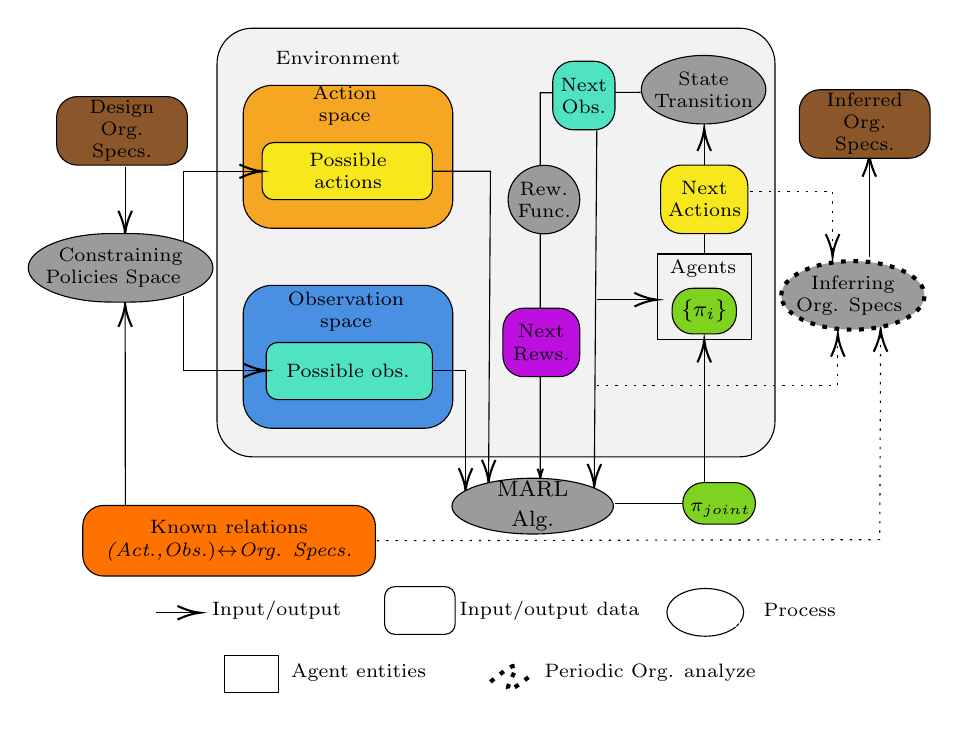
\begin{tikzpicture}[x=0.75pt,y=0.75pt,yscale=-1,xscale=1]
%uncomment if require: \path (0,1124); %set diagram left start at 0, and has height of 1124

%Shape: Rectangle [id:dp9937795244635512] 
\draw  [fill={rgb, 255:red, 242; green, 242; blue, 242 }  ,fill opacity=1 ] (108.97,721) .. controls (108.97,711.61) and (116.58,704) .. (125.97,704) -- (360.78,704) .. controls (370.17,704) and (377.78,711.61) .. (377.78,721) -- (377.78,893.49) .. controls (377.78,902.88) and (370.17,910.49) .. (360.78,910.49) -- (125.97,910.49) .. controls (116.58,910.49) and (108.97,902.88) .. (108.97,893.49) -- cycle ;
%Straight Lines [id:da6518751125509914] 
\draw    (335.62,932.92) -- (300.7,932.92) ;
%Straight Lines [id:da34207082497735786] 
\draw    (313,734.86) -- (264.7,735.09) -- (264.7,918.61) ;
\draw [shift={(264.7,920.61)}, rotate = 270] [color={rgb, 255:red, 0; green, 0; blue, 0 }  ][line width=0.75]    (4.37,-1.32) .. controls (2.78,-0.56) and (1.32,-0.12) .. (0,0) .. controls (1.32,0.12) and (2.78,0.56) .. (4.37,1.32)   ;
%Straight Lines [id:da9417034389402881] 
\draw    (343.7,754.18) -- (343.7,812.75) ;
\draw [shift={(343.7,752.18)}, rotate = 90] [color={rgb, 255:red, 0; green, 0; blue, 0 }  ][line width=0.75]    (10.93,-3.29) .. controls (6.95,-1.4) and (3.31,-0.3) .. (0,0) .. controls (3.31,0.3) and (6.95,1.4) .. (10.93,3.29)   ;
%Straight Lines [id:da4463435210078386] 
\draw    (343.7,922.88) -- (343.7,856.05) ;
\draw [shift={(343.7,854.05)}, rotate = 90] [color={rgb, 255:red, 0; green, 0; blue, 0 }  ][line width=0.75]    (10.93,-3.29) .. controls (6.95,-1.4) and (3.31,-0.3) .. (0,0) .. controls (3.31,0.3) and (6.95,1.4) .. (10.93,3.29)   ;
%Straight Lines [id:da8247669117759437] 
\draw    (291.96,834.78) -- (300.52,834.78) -- (318.99,834.78) ;
\draw [shift={(320.99,834.78)}, rotate = 180] [color={rgb, 255:red, 0; green, 0; blue, 0 }  ][line width=0.75]    (10.93,-3.29) .. controls (6.95,-1.4) and (3.31,-0.3) .. (0,0) .. controls (3.31,0.3) and (6.95,1.4) .. (10.93,3.29)   ;
%Rounded Rect [id:dp13052707912371297] 
\draw  [fill={rgb, 255:red, 245; green, 166; blue, 35 }  ,fill opacity=1 ] (121.59,745.3) .. controls (121.59,737.7) and (127.75,731.53) .. (135.35,731.53) -- (208.78,731.53) .. controls (216.39,731.53) and (222.55,737.7) .. (222.55,745.3) -- (222.55,786.6) .. controls (222.55,794.2) and (216.39,800.36) .. (208.78,800.36) -- (135.35,800.36) .. controls (127.75,800.36) and (121.59,794.2) .. (121.59,786.6) -- cycle ;
%Rounded Rect [id:dp7026077814365836] 
\draw  [fill={rgb, 255:red, 74; green, 144; blue, 226 }  ,fill opacity=1 ] (121.59,841.66) .. controls (121.59,834.06) and (127.75,827.89) .. (135.35,827.89) -- (208.78,827.89) .. controls (216.39,827.89) and (222.55,834.06) .. (222.55,841.66) -- (222.55,882.96) .. controls (222.55,890.56) and (216.39,896.72) .. (208.78,896.72) -- (135.35,896.72) .. controls (127.75,896.72) and (121.59,890.56) .. (121.59,882.96) -- cycle ;
%Rounded Rect [id:dp7429651229296941] 
\draw  [fill={rgb, 255:red, 248; green, 231; blue, 28 }  ,fill opacity=1 ] (130.7,764.57) .. controls (130.7,761.53) and (133.17,759.06) .. (136.21,759.06) -- (207.2,759.06) .. controls (210.24,759.06) and (212.7,761.53) .. (212.7,764.57) -- (212.7,781.09) .. controls (212.7,784.13) and (210.24,786.6) .. (207.2,786.6) -- (136.21,786.6) .. controls (133.17,786.6) and (130.7,784.13) .. (130.7,781.09) -- cycle ;
%Rounded Rect [id:dp2626666197665244] 
\draw  [fill={rgb, 255:red, 80; green, 227; blue, 194 }  ,fill opacity=1 ] (132.7,860.9) .. controls (132.7,857.86) and (135.17,855.39) .. (138.21,855.39) -- (207.2,855.39) .. controls (210.24,855.39) and (212.7,857.86) .. (212.7,860.9) -- (212.7,877.42) .. controls (212.7,880.46) and (210.24,882.92) .. (207.2,882.92) -- (138.21,882.92) .. controls (135.17,882.92) and (132.7,880.46) .. (132.7,877.42) -- cycle ;
%Straight Lines [id:da37906510942957117] 
\draw    (291.96,750.8) -- (290.72,922.92) ;
\draw [shift={(290.7,924.92)}, rotate = 270.41] [color={rgb, 255:red, 0; green, 0; blue, 0 }  ][line width=0.75]    (10.93,-3.29) .. controls (6.95,-1.4) and (3.31,-0.3) .. (0,0) .. controls (3.31,0.3) and (6.95,1.4) .. (10.93,3.29)   ;
%Straight Lines [id:da8878827995944159] 
\draw  [dash pattern={on 0.84pt off 2.51pt}]  (361.37,782.47) -- (405.54,782.47) -- (405.54,812.13) ;
\draw [shift={(405.54,814.13)}, rotate = 270] [color={rgb, 255:red, 0; green, 0; blue, 0 }  ][line width=0.75]    (10.93,-3.29) .. controls (6.95,-1.4) and (3.31,-0.3) .. (0,0) .. controls (3.31,0.3) and (6.95,1.4) .. (10.93,3.29)   ;
%Straight Lines [id:da8073435187842593] 
\draw  [dash pattern={on 0.84pt off 2.51pt}]  (291.96,876.08) -- (408.07,876.08) -- (408.07,853.3) ;
\draw [shift={(408.07,851.3)}, rotate = 90] [color={rgb, 255:red, 0; green, 0; blue, 0 }  ][line width=0.75]    (10.93,-3.29) .. controls (6.95,-1.4) and (3.31,-0.3) .. (0,0) .. controls (3.31,0.3) and (6.95,1.4) .. (10.93,3.29)   ;
%Straight Lines [id:da9521506867066192] 
\draw    (137.99,947.66) -- (64.8,947.66) -- (64.7,838.92) ;
\draw [shift={(64.7,836.92)}, rotate = 89.95] [color={rgb, 255:red, 0; green, 0; blue, 0 }  ][line width=0.75]    (10.93,-3.29) .. controls (6.95,-1.4) and (3.31,-0.3) .. (0,0) .. controls (3.31,0.3) and (6.95,1.4) .. (10.93,3.29)   ;
%Straight Lines [id:da8173351196218479] 
\draw  [dash pattern={on 0.84pt off 2.51pt}]  (177.06,950.92) -- (428.26,950.41) -- (428.69,850.92) ;
\draw [shift={(428.7,848.92)}, rotate = 90.25] [color={rgb, 255:red, 0; green, 0; blue, 0 }  ][line width=0.75]    (10.93,-3.29) .. controls (6.95,-1.4) and (3.31,-0.3) .. (0,0) .. controls (3.31,0.3) and (6.95,1.4) .. (10.93,3.29)   ;
%Straight Lines [id:da6053298376683525] 
\draw    (64.7,770.92) -- (64.7,800.92) ;
\draw [shift={(64.7,802.92)}, rotate = 270] [color={rgb, 255:red, 0; green, 0; blue, 0 }  ][line width=0.75]    (10.93,-3.29) .. controls (6.95,-1.4) and (3.31,-0.3) .. (0,0) .. controls (3.31,0.3) and (6.95,1.4) .. (10.93,3.29)   ;
%Straight Lines [id:da8641416537329594] 
\draw    (423.21,814.13) -- (423.21,766.57) ;
\draw [shift={(423.21,764.57)}, rotate = 90] [color={rgb, 255:red, 0; green, 0; blue, 0 }  ][line width=0.75]    (10.93,-3.29) .. controls (6.95,-1.4) and (3.31,-0.3) .. (0,0) .. controls (3.31,0.3) and (6.95,1.4) .. (10.93,3.29)   ;
%Shape: Rectangle [id:dp009612592743657444] 
\draw   (320.99,812.75) -- (366.42,812.75) -- (366.42,854.05) -- (320.99,854.05) -- cycle ;
%Shape: Boxed Line [id:dp9105440631185389] 
\draw    (79.7,985.61) -- (98.84,985.61) ;
\draw [shift={(100.84,985.61)}, rotate = 180] [color={rgb, 255:red, 0; green, 0; blue, 0 }  ][line width=0.75]    (10.93,-3.29) .. controls (6.95,-1.4) and (3.31,-0.3) .. (0,0) .. controls (3.31,0.3) and (6.95,1.4) .. (10.93,3.29)   ;
%Shape: Rectangle [id:dp18940852352890292] 
\draw   (112.7,1006.17) -- (138.7,1006.17) -- (138.7,1023.94) -- (112.7,1023.94) -- cycle ;
%Curve Lines [id:da6070406744312455] 
\draw [line width=1.5]  [dash pattern={on 1.69pt off 2.76pt}]  (240.7,1018.92) .. controls (271.17,993.71) and (230.78,1040.06) .. (261.24,1014.84) ;
%Straight Lines [id:da04181106466856366] 
\draw    (92.7,806.92) -- (92.7,772.92) -- (128.7,772.92) ;
\draw [shift={(130.7,772.92)}, rotate = 180] [color={rgb, 255:red, 0; green, 0; blue, 0 }  ][line width=0.75]    (10.93,-3.29) .. controls (6.95,-1.4) and (3.31,-0.3) .. (0,0) .. controls (3.31,0.3) and (6.95,1.4) .. (10.93,3.29)   ;
%Straight Lines [id:da5269327271789521] 
\draw    (92.7,832.92) -- (92.7,868.92) -- (130.7,868.92) ;
\draw [shift={(132.7,868.92)}, rotate = 180] [color={rgb, 255:red, 0; green, 0; blue, 0 }  ][line width=0.75]    (10.93,-3.29) .. controls (6.95,-1.4) and (3.31,-0.3) .. (0,0) .. controls (3.31,0.3) and (6.95,1.4) .. (10.93,3.29)   ;
%Straight Lines [id:da8384029096649059] 
\draw    (228.7,924.92) -- (228.7,868.92) -- (212.7,868.92) ;
\draw [shift={(228.7,926.92)}, rotate = 270] [color={rgb, 255:red, 0; green, 0; blue, 0 }  ][line width=0.75]    (10.93,-3.29) .. controls (6.95,-1.4) and (3.31,-0.3) .. (0,0) .. controls (3.31,0.3) and (6.95,1.4) .. (10.93,3.29)   ;
%Straight Lines [id:da8549749304566603] 
\draw    (212.7,772.92) -- (240.7,772.92) -- (239.8,920.92) ;
\draw [shift={(239.79,922.92)}, rotate = 270.35] [color={rgb, 255:red, 0; green, 0; blue, 0 }  ][line width=0.75]    (10.93,-3.29) .. controls (6.95,-1.4) and (3.31,-0.3) .. (0,0) .. controls (3.31,0.3) and (6.95,1.4) .. (10.93,3.29)   ;

% Text Node
\draw (177.2,1014.42) node  [font=\small] [align=left] {{\scriptsize Agent entities}};
% Text Node
\draw (317.7,1014.42) node  [font=\small] [align=left] {{\scriptsize Periodic Org. analyze}};
% Text Node
\draw    (189.7,978.02) .. controls (189.7,975.26) and (191.94,973.02) .. (194.7,973.02) -- (218.7,973.02) .. controls (221.46,973.02) and (223.7,975.26) .. (223.7,978.02) -- (223.7,991.02) .. controls (223.7,993.78) and (221.46,996.02) .. (218.7,996.02) -- (194.7,996.02) .. controls (191.94,996.02) and (189.7,993.78) .. (189.7,991.02) -- cycle  ;
\draw (206.7,984.52) node  [font=\small] [align=left] {\begin{minipage}[lt]{20.08pt}\setlength\topsep{0pt}
\begin{center}
\textcolor[rgb]{1,1,1}{{\tiny assaaaa}}
\end{center}

\end{minipage}};
% Text Node
\draw (269.2,984.42) node  [font=\small] [align=left] {{\scriptsize Input/output data}};
% Text Node
\draw (137.7,984.42) node  [font=\small] [align=left] {{\scriptsize Input/output}};
% Text Node
\draw    (325.7,985.42) .. controls (325.7,979.07) and (333.98,973.92) .. (344.2,973.92) .. controls (354.42,973.92) and (362.7,979.07) .. (362.7,985.42) .. controls (362.7,991.77) and (354.42,996.92) .. (344.2,996.92) .. controls (333.98,996.92) and (325.7,991.77) .. (325.7,985.42) -- cycle  ;
\draw (344.2,985.42) node  [font=\small] [align=left] {\begin{minipage}[lt]{22.12pt}\setlength\topsep{0pt}
\begin{center}
\textcolor[rgb]{1,1,1}{{\tiny aassssaa}}
\end{center}

\end{minipage}};
% Text Node
\draw (389.7,984.42) node  [font=\small] [align=left] {{\scriptsize Process}};
% Text Node
\draw  [fill={rgb, 255:red, 139; green, 87; blue, 42 }  ,fill opacity=1 ]  (31.7,746.92) .. controls (31.7,741.4) and (36.18,736.92) .. (41.7,736.92) -- (84.7,736.92) .. controls (90.22,736.92) and (94.7,741.4) .. (94.7,746.92) -- (94.7,759.92) .. controls (94.7,765.45) and (90.22,769.92) .. (84.7,769.92) -- (41.7,769.92) .. controls (36.18,769.92) and (31.7,765.45) .. (31.7,759.92) -- cycle  ;
\draw (63.2,753.42) node  [font=\scriptsize] [align=left] {\begin{minipage}[lt]{40.43pt}\setlength\topsep{0pt}
\begin{center}
Design\\Org. Specs.
\end{center}

\end{minipage}};
% Text Node
\draw  [fill={rgb, 255:red, 155; green, 155; blue, 155 }  ,fill opacity=1 ]  (249.21,786.55) .. controls (249.21,777.43) and (256.94,770.05) .. (266.46,770.05) .. controls (275.99,770.05) and (283.72,777.43) .. (283.72,786.55) .. controls (283.72,795.66) and (275.99,803.05) .. (266.46,803.05) .. controls (256.94,803.05) and (249.21,795.66) .. (249.21,786.55) -- cycle  ;
\draw (266.46,786.55) node  [font=\scriptsize,xslant=-0.02] [align=left] {\begin{minipage}[lt]{20.58pt}\setlength\topsep{0pt}
\begin{center}
Rew.\\Func.
\end{center}

\end{minipage}};
% Text Node
\draw (165.76,716.05) node  [font=\scriptsize] [align=left] {\begin{minipage}[lt]{42.81pt}\setlength\topsep{0pt}
\begin{center}
Environment
\end{center}

\end{minipage}};
% Text Node
\draw (170.49,741.51) node  [font=\scriptsize] [align=left] {\begin{minipage}[lt]{43.61pt}\setlength\topsep{0pt}
\begin{center}
Action space
\end{center}

\end{minipage}};
% Text Node
\draw (171.12,840.63) node  [font=\scriptsize] [align=left] {\begin{minipage}[lt]{62.26pt}\setlength\topsep{0pt}
\begin{center}
Observation space
\end{center}

\end{minipage}};
% Text Node
\draw (172.07,772.83) node  [font=\scriptsize] [align=left] {\begin{minipage}[lt]{54.32pt}\setlength\topsep{0pt}
\begin{center}
Possible actions
\end{center}

\end{minipage}};
% Text Node
\draw (172.07,869.19) node  [font=\scriptsize] [align=left] {\begin{minipage}[lt]{45.19pt}\setlength\topsep{0pt}
\begin{center}
Possible obs.
\end{center}

\end{minipage}};
% Text Node
\draw  [fill={rgb, 255:red, 155; green, 155; blue, 155 }  ,fill opacity=1 ]  (261.04, 934.24) circle [x radius= 38.89, y radius= 13.44]   ;
\draw (261.04,934.24) node  [font=\small] [align=left] {\begin{minipage}[lt]{37.13pt}\setlength\topsep{0pt}
\begin{center}
{\footnotesize MARL Alg.}
\end{center}

\end{minipage}};
% Text Node
\draw  [fill={rgb, 255:red, 126; green, 211; blue, 33 }  ,fill opacity=1 ]  (333.36,932.92) .. controls (333.36,927.4) and (337.84,922.92) .. (343.36,922.92) -- (358.36,922.92) .. controls (363.88,922.92) and (368.36,927.4) .. (368.36,932.92) .. controls (368.36,938.45) and (363.88,942.92) .. (358.36,942.92) -- (343.36,942.92) .. controls (337.84,942.92) and (333.36,938.45) .. (333.36,932.92) -- cycle  ;
\draw (350.86,932.92) node  [font=\scriptsize] [align=left] {\begin{minipage}[lt]{20.95pt}\setlength\topsep{0pt}
\begin{center}
$\displaystyle \pi _{joint}$
\end{center}

\end{minipage}};
% Text Node
\draw  [fill={rgb, 255:red, 155; green, 155; blue, 155 }  ,fill opacity=1 ]  (313.39,733.6) .. controls (313.39,724.48) and (326.82,717.1) .. (343.39,717.1) .. controls (359.96,717.1) and (373.39,724.48) .. (373.39,733.6) .. controls (373.39,742.71) and (359.96,750.1) .. (343.39,750.1) .. controls (326.82,750.1) and (313.39,742.71) .. (313.39,733.6) -- cycle  ;
\draw (343.39,733.6) node  [font=\scriptsize] [align=left] {\begin{minipage}[lt]{37.77pt}\setlength\topsep{0pt}
\begin{center}
State\\Transition \ 
\end{center}

\end{minipage}};
% Text Node
\draw  [fill={rgb, 255:red, 189; green, 16; blue, 224 }  ,fill opacity=1 ]  (246.7,848.88) .. controls (246.7,843.35) and (251.18,838.88) .. (256.7,838.88) -- (273.7,838.88) .. controls (279.22,838.88) and (283.7,843.35) .. (283.7,848.88) -- (283.7,861.88) .. controls (283.7,867.4) and (279.22,871.88) .. (273.7,871.88) -- (256.7,871.88) .. controls (251.18,871.88) and (246.7,867.4) .. (246.7,861.88) -- cycle  ;
\draw (265.2,855.38) node  [font=\scriptsize] [align=left] {\begin{minipage}[lt]{22.57pt}\setlength\topsep{0pt}
\begin{center}
Next\\Rews.
\end{center}

\end{minipage}};
% Text Node
\draw  [fill={rgb, 255:red, 255; green, 114; blue, 0 }  ,fill opacity=1 ]  (44.27,943.92) .. controls (44.27,938.4) and (48.75,933.92) .. (54.27,933.92) -- (175.27,933.92) .. controls (180.79,933.92) and (185.27,938.4) .. (185.27,943.92) -- (185.27,957.92) .. controls (185.27,963.45) and (180.79,967.92) .. (175.27,967.92) -- (54.27,967.92) .. controls (48.75,967.92) and (44.27,963.45) .. (44.27,957.92) -- cycle  ;
\draw (114.77,950.92) node  [font=\scriptsize] [align=left] {\begin{minipage}[lt]{93.15pt}\setlength\topsep{0pt}
\begin{center}
Known relations\\\textit{(Act.,Obs.})$\displaystyle \leftrightarrow $\textit{Org. Specs.}
\end{center}

\end{minipage}};
% Text Node
\draw  [fill={rgb, 255:red, 155; green, 155; blue, 155 }  ,fill opacity=1 ]  (18,819.42) .. controls (18,810.31) and (35.91,802.92) .. (58,802.92) -- (67,802.92) .. controls (89.09,802.92) and (107,810.31) .. (107,819.42) .. controls (107,828.54) and (89.09,835.92) .. (67,835.92) -- (58,835.92) .. controls (35.91,835.92) and (18,828.54) .. (18,819.42) -- cycle  ;
\draw (62.5,819.42) node  [font=\scriptsize] [align=left] {\begin{minipage}[lt]{57.49pt}\setlength\topsep{0pt}
\begin{center}
Constraining\\Policies Space \ \ \ 
\end{center}

\end{minipage}};
% Text Node
\draw  [fill={rgb, 255:red, 80; green, 227; blue, 194 }  ,fill opacity=1 ]  (270.7,729.92) .. controls (270.7,724.4) and (275.18,719.92) .. (280.7,719.92) -- (290.7,719.92) .. controls (296.22,719.92) and (300.7,724.4) .. (300.7,729.92) -- (300.7,742.92) .. controls (300.7,748.45) and (296.22,752.92) .. (290.7,752.92) -- (280.7,752.92) .. controls (275.18,752.92) and (270.7,748.45) .. (270.7,742.92) -- cycle  ;
\draw (285.7,736.42) node  [font=\scriptsize] [align=left] {\begin{minipage}[lt]{17.81pt}\setlength\topsep{0pt}
\begin{center}
Next\\Obs.
\end{center}

\end{minipage}};
% Text Node
\draw (343.14,819.98) node  [font=\scriptsize] [align=left] {\begin{minipage}[lt]{24.96pt}\setlength\topsep{0pt}
\begin{center}
Agents
\end{center}

\end{minipage}};
% Text Node
\draw  [fill={rgb, 255:red, 126; green, 211; blue, 33 }  ,fill opacity=1 ]  (328.2,839.28) .. controls (328.2,833.76) and (332.68,829.28) .. (338.2,829.28) -- (349.2,829.28) .. controls (354.73,829.28) and (359.2,833.76) .. (359.2,839.28) -- (359.2,841.28) .. controls (359.2,846.81) and (354.73,851.28) .. (349.2,851.28) -- (338.2,851.28) .. controls (332.68,851.28) and (328.2,846.81) .. (328.2,841.28) -- cycle  ;
\draw (343.7,840.28) node  [font=\footnotesize] [align=left] {\begin{minipage}[lt]{18.45pt}\setlength\topsep{0pt}
\begin{center}
$\displaystyle \{\pi _{i}\}$
\end{center}

\end{minipage}};
% Text Node
\draw  [fill={rgb, 255:red, 248; green, 231; blue, 28 }  ,fill opacity=1 ]  (322.7,779.92) .. controls (322.7,774.4) and (327.18,769.92) .. (332.7,769.92) -- (354.7,769.92) .. controls (360.22,769.92) and (364.7,774.4) .. (364.7,779.92) -- (364.7,792.92) .. controls (364.7,798.45) and (360.22,802.92) .. (354.7,802.92) -- (332.7,802.92) .. controls (327.18,802.92) and (322.7,798.45) .. (322.7,792.92) -- cycle  ;
\draw (343.7,786.42) node  [font=\scriptsize] [align=left] {\begin{minipage}[lt]{26.14pt}\setlength\topsep{0pt}
\begin{center}
Next\\Actions
\end{center}

\end{minipage}};
% Text Node
\draw  [color={rgb, 255:red, 0; green, 0; blue, 0 }  ,draw opacity=1 ][fill={rgb, 255:red, 155; green, 155; blue, 155 }  ,fill opacity=1 ][dash pattern={on 1.69pt off 2.76pt}][line width=1.5]   (380.82,832.71) .. controls (380.82,823.6) and (396.27,816.21) .. (415.32,816.21) .. controls (434.38,816.21) and (449.82,823.6) .. (449.82,832.71) .. controls (449.82,841.82) and (434.38,849.21) .. (415.32,849.21) .. controls (396.27,849.21) and (380.82,841.82) .. (380.82,832.71) -- cycle  ;
\draw (415.32,832.71) node  [font=\scriptsize] [align=left] {\begin{minipage}[lt]{44.39pt}\setlength\topsep{0pt}
\begin{center}
Inferring\\Org. Specs \ \ 
\end{center}

\end{minipage}};
% Text Node
\draw  [fill={rgb, 255:red, 139; green, 87; blue, 42 }  ,fill opacity=1 ]  (389.5,743.62) .. controls (389.5,738.09) and (393.98,733.62) .. (399.5,733.62) -- (442.5,733.62) .. controls (448.02,733.62) and (452.5,738.09) .. (452.5,743.62) -- (452.5,756.62) .. controls (452.5,762.14) and (448.02,766.62) .. (442.5,766.62) -- (399.5,766.62) .. controls (393.98,766.62) and (389.5,762.14) .. (389.5,756.62) -- cycle  ;
\draw (421,750.12) node  [font=\scriptsize] [align=left] {\begin{minipage}[lt]{40.43pt}\setlength\topsep{0pt}
\begin{center}
Inferred\\Org. Specs.
\end{center}

\end{minipage}};


\end{tikzpicture}
  \caption{Une vue récapitulative du processus PRAHOM}
  \label{fig:prahom_process}
\end{figure}

\paragraph{\textbf{Déduire des spécifications organisationnelles}}

Plutôt que d'utiliser directement les politiques conjointes, nous utilisons les historiques conjoints car ils peuvent être construits avec les actions résultantes observées lorsque les observations sont reçues au cours d'une série d'épisodes de test. En effet, pour une politique donnée $\pi \in \Pi$, l'historique associé est par définition $h \in h_{joint} = \langle(\omega_k,a_k) | k \in \mathbb{N}\rangle$ et le $(\omega_k,a_k) \in \pi$.
Ensuite, en raison de la difficulté de déduire des informations liées aux spécifications organisationnelles, il est possible d'associer chaque observation ou action aux spécifications de l'organisation sous la forme d'une relation \textquote{plusieurs à plusieurs}. Cela met en place un premier cadre d’identification des spécifications organisationnelles dans les historiques. Nous abordons ce problème dans le reste de cette section.

On peut définir certaines relations entre les spécifications $\mathcal{M}OISE^+$ et les historiques conjoints. Leurs prémisses viennent du fait que certaines spécifications du modèle organisationnel $\mathcal{M}OISE^+$ peuvent être mappées à des sous-ensembles d'actions d'une seule politique commune sous-optimale.
À partir de ces relations, il est possible d’utiliser des approches empiriques ou statistiques pour déduire des spécifications organisationnelles à partir d’historiques communes. Ci-dessous, nous décrivons de manière informelle les points clés pour comprendre ce processus.

Comme nous n’avons qu’un seul groupe, nous ne considérons pas les inter-liens et les inter-compatibilités. De plus, par souci de simplification, nous ne considérons qu’un seul schème social.
Premièrement, nous examinons le niveau individuel en essayant de comprendre les rôles, les liens, les sous-groupes, les objectifs individuels, les missions et les plans joués par les agents en échantillonnant les sous-séquences historiques $h \in H$ et en les comparant avec les sous-séquences historiques connues dont nous avons besoin. connaître le rôle associé via les relations établies.

Après avoir analysé plusieurs politiques communes, nous essayons de renforcer une vision globale des objectifs, des missions, des plans et de la connaissance de la mission par rapport à l'objectif ; avec les informations partiellement déduites au niveau individuel.
Au final, notre processus tente de synthétiser les connaissances inférées jusqu'à avoir une meilleure vision de la cardinalité des agents par sous-groupe, de la cardinalité des agents pour chaque mission, de la cardinalité des rôles, des compatibilités entre rôles, des autorisations et des obligations.

\paragraph{\textbf{Contraindre l'espace des politiques}}

Nous considérons un algorithme MARL donné qui converge itérativement vers une politique commune de sorte que la politique de chaque agent soit mise à jour à chaque étape jusqu'à un horizon fini.
Nous avons privilégié l'algorithme \emph{Proximal Policy Optimization} pour son efficacité prouvée dans des environnements multi-agents coopératifs sans nécessiter de modifications algorithmiques ou d'architectures spécifiques au domaine~\cite{Yu2022}.
Pour contraindre les politiques conjointes possibles à celles satisfaisant les spécifications organisationnelles de conception $os_{init}$, nous proposons de contraindre les ensembles d'actions et d'observations pour chaque agent en fonction de $os_{init}$ à chaque étape. Par exemple, nous pouvons contraindre un agent à converger vers un rôle donné en interdisant les actions liées à d’autres rôles. Nous avons utilisé cette idée pour mettre en place notre processus visant à guider l'entrainement en fonction de certaines contraintes organisationnelles de conception.

Dans un premier temps, nous utilisons les relations précédemment établies entre spécifications organisationnelles et couples action-observation, pour déterminer les actions autorisées ou interdites jouables par les agents à chaque étape.
Ensuite, il calcule d'abord l'ensemble d'actions autorisées $A_{step}$ en fonction de l'historique actuel $h_{joint,i}$. Ensuite, une action est choisie parmi les actions autorisées. Cette action $a_{step} \in A_{step}$ est ajoutée à l'historique pour être utilisée pour mettre à jour la politique de l'agent à l'étape suivante. Ensuite, l'algorithme MARL met à jour la politique commune, donc les politiques des agents, avec l'action et l'observation en cours.
Enfin, une analyse de la politique conjointe sous-optimale actuelle $\pi_{joint}$ satisfaisant $os_{init}$ est déclenchée périodiquement. Il permet d’améliorer de manière itérative l’efficacité des politiques conjointes et l’exactitude des spécifications organisationnelles qui en découlent.
Nous pouvons noter que la restriction impliquée par $os_{init}$ dans les éventuelles politiques conjointes pourrait empêcher l'algorithme MARL de trouver une politique commune qui satisfasse la récompense cumulative minimale attendue définie par le concepteur.

\subsection{Outil d'ingénierie}

PettingZoo est une bibliothèque qui propose une API standardisée qui simplifie le développement d'environnements avec des agents et facilite l'application des algorithmes MARL.
Nous avons développé \emph{PRAHOM PettingZoo Wrapper}\label{PettingZoo-wrapper}, un outil pour aider à automatiser la configuration de \emph{PRAHOM} pour un environnement PettingZoo donné.
Il s'agit d'une Preuve de Concept qui permet de relier les actions aux spécifications $\mathcal{M}OISE^+$ et de définir les spécifications organisationnelles. Il fournit des fonctions pour extraire les spécifications organisationnelles brutes sous-optimales qui en résultent. Lors de l'entrainement, des actions sont masquées pour guider un agent à apprendre à agir selon les spécifications organisationnelles.

\begin{lstlisting}[language=Python, caption=PRAHOM PettingZoo Wrapper basic use, label={lst:wrapper_basic_use}]
from omarl_experiments import PrahomWrapper
env = PettingZoo_env.parallel_env(render_mode="human")
...
action_to_specs = {"agent_name": {
        "14": "role='leader';link='(agent_0,agent_1,auth);..."
        ...}    
    ...}
training_specs = {
    "leadadversary_0": {
        "must": ["(23,41)"],
        "must_not": ["(14,74)"]}...}
env = PrahomWrapper(env, action_to_specs, training_specs, unknown_specs_inference=True, pca_output=True)
# ...TRAINING...
env.prahom_render_pca()
trained_specs, agent_to_specs = env.prahom_specs()
\end{lstlisting}

Dans \autoref{lst:wrapper_basic_use}, nous avons détaillé une utilisation basique du wrapper pour augmenter un environnement PettingZoo (l.12) avec des relations connues entre les actions et les spécifications organisationnelles (l.4) et les contraintes de conception que les agents doivent satisfaire (l.8). Après l'entrainement, nous pouvons afficher une Analyse en Composantes Principales (ACP) de l'historique de chaque agent sur un épisode (l.14) qui est un outil d'analyse supplémentaire pour détecter manuellement les rôles émergents. Il fournit également les spécifications $\mathcal{M}OISE^+$ déduites en tenant compte des derniers épisodes et de la manière dont les agents sont instanciés dans le dernier épisode.

Ces résultats sont construits via des approches empiriques ou statistiques en utilisant les relations connues entre les observations, les actions et les spécifications organisationnelles. Lorsqu'aucune relation n'est disponible, il tente de détecter des sous-séquences d'historiques communes susceptibles de correspondre à une spécification organisationnelle (l. 12). En raison de ces limitations, les résultats peuvent ne pas décrire entièrement l’organisation sous-jacente ou contenir des spécifications organisationnelles déduites bruyantes. Puisque les résultats sont conformes à $\mathcal{M}OISE^+$, il est alors possible de les utiliser avec les méthodes de conception SMA disponibles pour bénéficier des spécifications organisationnelles émergentes identifiées au cours du processus de conception.

% =============

% \begin{itemize}
% \item Questions au niveau du système multi-agents (approche centrée sur le système)
% \begin{itemize}
% \item Nombre d'agents, quelle hétérogénéité ?
% \item Quel est le support commun (Environnement) partagé par les agents ?
% \item Quels mécanismes de communication sont disponibles pour les agents ?
% \item Quels sont les langages de communication, les ontologies, les protocoles d'interaction utilisés par les agents ?
% \item Quelle est l’organisation au sein de laquelle les agents opèrent ? Comment est-il établi ?
% \item Comment les agents coordonnent-ils leurs actions ? Comment assurer un fonctionnement cohérent ?
% \end{itemize}

% \item Questions au niveau de l'agent (approche centrée sur l'agent)
% \begin{itemize}
% \item Que représente un agent ? Quelles actions doivent être encapsulées dans un agent ?
% \item Comment les agents représentent-ils l'environnement et l'organisation dans lesquels ils opèrent ?
% \item Comment les agents gèrent-ils les interactions avec d'autres agents ?
% \item Quelle est la structure interne des agents ?
% \end{itemize}
% \end{itemize}

% ================================================== =================================================== =

\section{Évaluation dans des environnements de jeu coopératif}

% Évaluation
% Afin de vérifier et démontrer l'approche, est appliquée sur l'étude de cas suivante.
% 	Étude de cas

Afin d'évaluer AOMEA, nous avons envisagé d'utiliser \emph{PRAHOM} dans des environnements simulés disponibles composés d'agents devant atteindre un objectif avec les meilleures performances à travers diverses stratégies collectives dont certaines peuvent être facilement comprises.
Nous avons sélectionné trois environnements de type Atari pour leur rendu visuel qui constitue un moyen pratique d'évaluer les résultats avec des observations manuelles\footnotemark[1].
Nous avons également considéré un environnement de Cyberdéfense comme une première tentative d'application de \emph{PRAHOM} dans un environnement de Cyberdéfense non visuel :

\footnotetext[1]{Des explications supplémentaires et les exemples discutés utilisant le \emph{PRAHOM PettingZoo wrapper} sont disponibles sur \url{https://github.com/julien6/omarl_experiments?tab=readme-ov-file\#tutorial-predator-prey-with-communication}}

\begin{itemize}
  \item \textquote{Drone swarm - 3rd CAGE Challenge}~\cite{cage_challenge_3_announcement} (CYB) se compose d'agents cyberdender déployés sur des drones en réseau essayant de lutter contre les programmes malware déployés de manière malveillante. Nous pouvons nous attendre à ce que les agents \allowbreak isolent collectivement les drones compromis ;
  \item \textquote{Pistonball} (PBL)~\cite{Terry2021} se compose d'une série de pistons pour amener une balle de droite à gauche, nécessitant ainsi la représentation des voisins ;
  \item \textquote{Predator-prey with communication}~\cite{Lowe2017} (PPY) se compose de prédateurs surveillés par un leader pour mieux attraper des proies plus rapides, nécessitant ainsi des stratégies de chasse collectives ;
  \item \textquote{Knights Archers Zombies}~\cite{Terry2021} (KAZ) consiste en trois chevaliers et deux archers apprenant à tuer le plus de zombies ce qui nécessite ainsi un positionnement spatial efficace des agents.
\end{itemize}

Nous avons appliqué AOMEA dans trois cas :
\begin{itemize}
  \item Pas de spécifications organisationnelles (NTS) : les agents doivent apprendre les stratégies collectives les plus efficaces sans aucune contrainte ni indication.
  \item Spécifications organisationnelles partiellement contraignantes (PTS) : certaines contraintes ou indications sont données pour aider à converger plus rapidement ou à répondre à des exigences.
  \item Spécifications organisationnelles entièrement contraignantes (FTS) : des politiques conjointes élaborées manuellement sont données car elles constituent une référence concernant les politiques conjointes apprises.
\end{itemize}

Ici, nous ne présentons pas le détail des contraintes données dans NTS et FTS (disponibles dans le référentiel Git\footnotemark[1]).

\begin{figure}[h!]
  \centering
  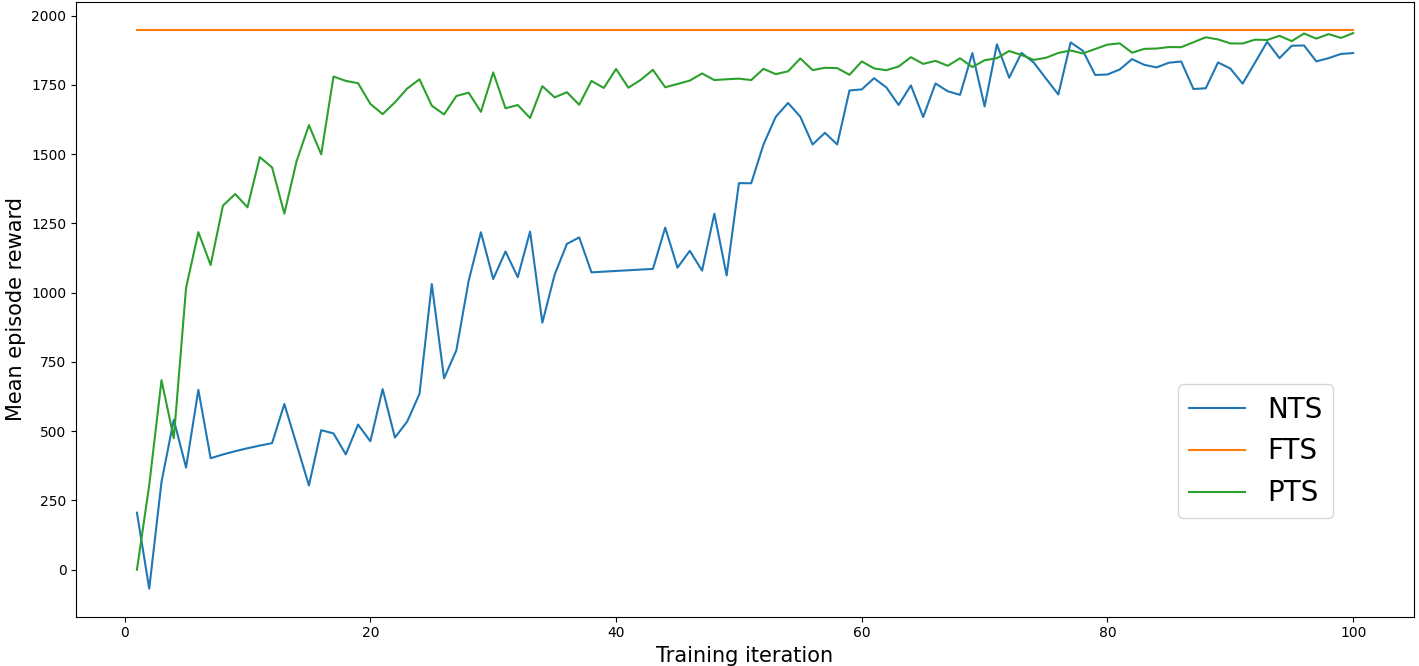
\includegraphics[width=\linewidth]{figures/prahom_learning_curve.png}
  \caption{Récompense moyenne pour chaque itération dans l'environnement PBL pour les cas NTS, PTS et FTS}
  \label{fig:prahom_learning_curve}
\end{figure}

\begin{figure}[h!]
  \centering
  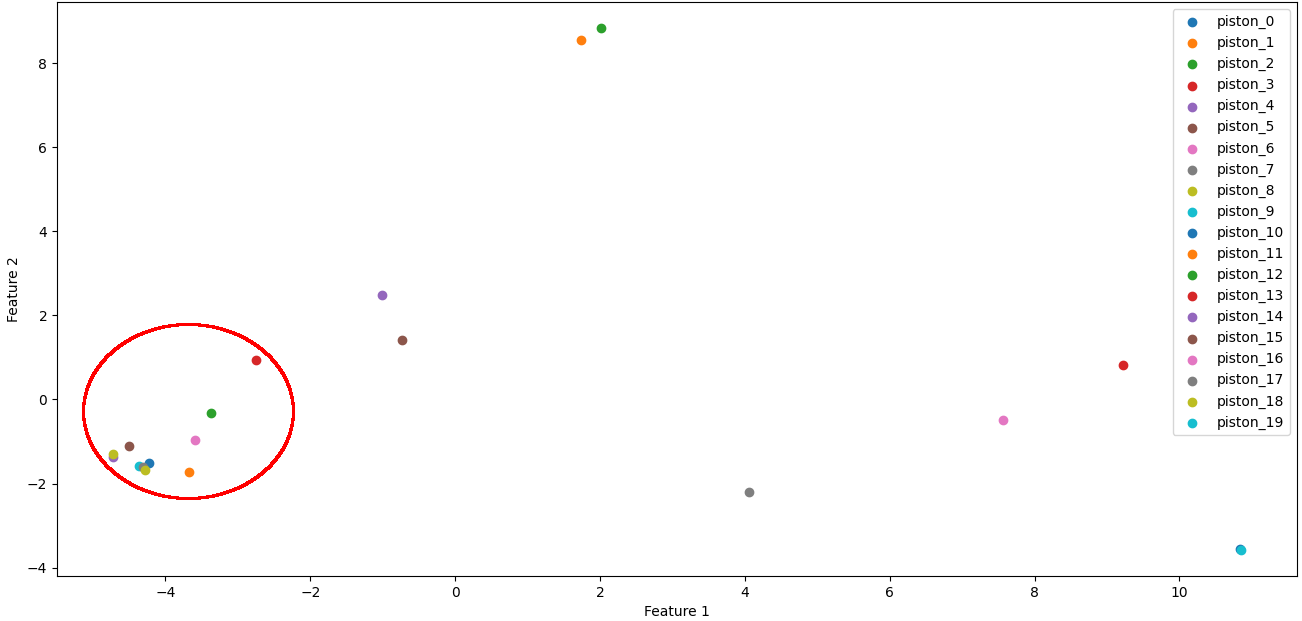
\includegraphics[width=\linewidth]{figures/prahom_pca_analysis.png}
  \caption{ACP des historiques des agents entrainés dans l'environnement PBL}
  \label{fig:prahom_pca_analysis}
\end{figure}

Nous évaluons l'impact de \emph{PRAHOM} sur les critères suivants : les ratios de temps de convergence entre PTS, NTS et FTS pour atteindre un seuil de récompense cumulée. La stabilité des performances montre comment les agents entrainés peuvent atteindre l'objectif de façon générale en évaluant plusieurs environnements générés avec différents paramètres. Les résultats sont présentés dans le tableau~\ref{tab:training_AOMEA_results}.
%
\begin{table}[t!]

    \centering

    \begin{tblr}{colspec={llll},rows={m},measure=vbox,stretch=-1}

        \textbf{Environment} & \textbf{PTS/NTS} & \textbf{PTS/FTS} & \textbf{Perf. stability \\ (avg. / max)} \\

        \hline

        { PPL }
        & { 4.7 }
        & { 1.3 }
        & { 0.9 } \\

        \hline[dashed]

        { PPY }
        & { 6.3 }
        & { 2.2 }
        & { 0.78 } \\

        \hline[dashed]

        { KAZ }
        & { 4.0 }
        & { 1.1 }
        & { 0.42 } \\

        \hline[dashed]

        { CYB }
        & { 12 }
        & { 3.3 }
        & { 0.36 } \\


    \end{tblr}

    \caption{View of the AOMEA approach impact during training}

    \label{tab:training_AOMEA_results}

\end{table}

%
De manière générale, on peut remarquer que le temps de convergence est plus long pour NTS que pour PTS qui est également plus long que pour FTS. Comme prévu, l’espace de recherche diminue, d’où un temps de convergence plus court. Par exemple, nous avons remarqué une convergence plus rapide vers une solution sous-optimale dans l’environnement PBL en fournissant des spécifications organisationnelles telles que présentées dans \autoref{fig:prahom_learning_curve}. Bien que le PTS converge plus rapidement que le NTS vers une récompense cumulée comparable, le NTS peut surpasser le PTS parce que les politiques des agents entrainés sont conçues sur mesure pour résoudre le problème de manière beaucoup plus fine que ne le peuvent les spécifications organisationnelles du concepteur. Une faible stabilité des performances dans l'environnement CYB plus complexe indique que les agents entrainés ont des difficultés à trouver des stratégies générales par rapport aux agents des autres environnements.

Nous avons également pris en compte les critères suivants après l'entrainement : rôles, liens et performance globale. Une analyse qualitative est présentée dans le tableau~\ref{tab:trained_AOMEA_results}
%
\begin{table}[t!]

    \centering

    \begin{tblr}{colspec={llll},rows={m},measure=vbox,stretch=-1}

        \textbf{Environment} & \textbf{Roles} & \textbf{Links} & \textbf{Global performance} \\

        \hline

        { 1 }
        & {  }
        & {  } \\
        & {  } \\

        \hline[dashed]

        { 2 }
        & {  }
        & {  } \\
        & {  } \\

        \hline[dashed]

        { 3 }
        & {  }
        & {  } \\
        & {  } \\

        \hline[dashed]

        { 4 }
        & {  }
        & {  } \\
        & {  } \\

        \hline[dashed]

        { 5 }
        & {  }
        & {  } \\
        & {  } \\

    \end{tblr}

    \caption{View of the OOMARL approach impact after training}

    \label{tab:trained_OOMARL_results}

\end{table}

%
% //TODO : schémas Moise+ et comparaison avec ceux attendus
%
Pour l'environnement PBL, nous pouvons remarquer que les rôles sont équivalents car les agents sont censés agir de la même manière. En effet, les historiques des agents entrainés sont proches, montrant ainsi un rôle émergent commun. Nous avons généré l'ACP présentée dans \autoref{fig:prahom_pca_analysis} en exprimant les historiques des agents sous forme de vecteurs contenant les couples observation-action. Nous pouvons remarquer que l'historique de la plupart des agents se trouve dans la zone inférieure gauche (encerclée en rouge). Cela montre que la plupart des pistons semblent agir de la même manière que prévu. Nous n'observons aucune spécification organisationnelle mis à part les rôles générés car les agents ne peuvent pas communiquer. Pour l'environnement KAZ, on peut remarquer deux rôles distincts : les archers ont tendance à s'éloigner des zombies, tandis que les chevaliers ont tendance à s'en approcher. Pour l'environnement PPY, nous pouvons observer que les spécifications de sortie indiquent des liens d'autorité entre le prédateur leader et les prédateurs simples pour permettre des stratégies collectives pour encercler les proies. Enfin, l’environnement CYB montre que les communications entre agents bleus sont bien comprises comme des liens de communication permettant d’isoler les drones infiltrés ou de tenter de réparer et d’alerter les drones récemment suspectés.

Pour l'environnement CYB, nous avons développé notre SMA raffiné via un simple arbre de décision élaboré à la main tel que préconisé dans AOMEA à la lumière des spécifications organisationnelles que nous avons obtenues en supprimant le bruit. Notre approche ne suggère pas de rôles généraux, mais des modèles stratégiques pertinents ont été identifiés. Par exemple, concernant les liens entre les rôles des agents, nous avons remarqué que les agents qui envoient des messages semblent fréquemment repérés comme suspects par leurs voisins. De plus, un agent cyber-défenseur se trouvant dans le rayon de communication d’un drone suspecté a tendance à couper sa communication et à la réactiver par la suite. Même si ces informations sont peu nombreuses, le score moyen que nous avons obtenu avec notre SMA affiné est d'environ -2000, ce qui est en effet proche des 5 meilleurs scores. Cela montre qu'AOMEA est effectivement applicable au contexte de la cyberdéfense, apportant en outre des garanties de sécurité.

\section{Conclusion}

% Dans cet article, nous avons présenté AOMEA, une nouvelle approche générale de conception SMA qui vise à faciliter la conception SMA lorsqu'elle ne peut pas être facilement réalisée par les concepteurs dans des environnements de déploiement très complexes.
Les travaux méthodologiques du SMA s'appuient sur les connaissances du concepteur pour concevoir une organisation SMA adaptée mais ne fournissent pas de moyens automatiques ou assistés pour déterminer les mécanismes organisationnels pertinents.
% uniquement à partir des exigences de conception et de l'objectif global.
Les techniques MARL ont été appliquées avec succès pour entrainer automatiquement des agents à atteindre un objectif donné sans caractérisation explicite des stratégies collectives émergentes.
L'originalité d'AOMEA est d'enrichir un processus MARL d'un modèle organisationnel explicite vers un objectif méthodologique pour aborder ces problématiques. Nous avons d'abord exposé comment AOMEA est destiné à être utilisé dans l'ingénierie SMA en tant qu'outil supplémentaire pour aider au processus de conception.
Ensuite, nous avons expliqué le noyau théorique d'AOMEA avec les liens entre Dec-POMDP et le $\mathcal{M}OISE^+$ à travers le processus \emph{PRAHOM}.
De plus, nous avons implémenté le wrapper \emph{PRAHOM PettingZoo} comme preuve de concept pour appliquer pratiquement AOMEA et nous avons montré qu'il permet d'obtenir des spécifications organisationnelles qui satisfont aux contraintes de conception et permettent d'atteindre l'objectif donné.
Enfin, nous avons appliqué notre approche dans quatre environnements PettingZoo pour évaluer l'impact pendant et après l'entrainement. Les résultats de performance obtenus se révèlent comparables à ceux connus, démontrant que notre approche est viable.

Même si \emph{PRAHOM} est agnostique à l'égard de l'algorithme MARL car il utilise l'historique des agents pour déduire des spécifications organisationnelles, reconstruire a posteriori les comportements collectifs des agents peut s'avérer difficile. En effet, une perspective majeure pour améliorer \emph{PRAHOM} est d'aller plus loin avec les techniques d'apprentissage supervisé et non supervisé en plus des approches statistiques empiriques pour identifier des spécifications organisationnelles pertinentes à partir d'historiques conjointes. De plus, il vaut la peine d’étudier les travaux récents sur les techniques MARL telles que l’apprentissage hiérarchique car ils cherchent déjà à caractériser les stratégies émergentes tout au long de l’apprentissage.
%À terme, nous visons également à améliorer l'applicabilité d'AOMEA en développant des interfaces dédiées construites autour de \emph{PRAHOM} le rendant plus accessible aux contextes industriels et de recherche.


% \begin{thebibliography}{9}
% {\small
% \bibitem{bar} U. Nexpert, \emph{Le livre,} Son Editeur, 1929.

% \bibitem{foo} I. Troiseu-Pami, Un article intéressant, \emph{Journal de
%     Spirou}, Vol. 17, pp. 1-100, 1987
% }
% \end{thebibliography}

\bibliographystyle{plain}
\bibliography{references}

\end{document}

%%% Local Variables: 
%%% mode: latex
%%% TeX-SMAter: "jfsmaLatex"
%%% ispell-local-dictionary: "francais"
%%% TeX-command-extra-options: "-shell-escape"
%%% End: 